% =====================================================================
%  Capitolo 17 — L'interior design per il level designer: l'ordine
%  (pattern, ricorrenza e contrasto, orientamento, spazi espliciti e
%  impliciti) (Game Design, primo anno)
%  Fonte: trascrizione della lezione GD17, quarta lezione del corso di
%  Level Design del primo anno (docente: Stefano Zocchi, lo stesso dei
%  capitoli 8, 11 e 14), di cui è la diretta prosecuzione: i task
%  rivisti in apertura sono le stanze "illuminate con uno scopo"
%  assegnate nel capitolo 14. Lezione tenuta in streaming da casa del
%  docente (il primo streaming "da questo computer"), in un giorno
%  diverso dal solito.
%  Contenuti, nell'ordine della lezione: le prove tecniche dello
%  streaming; la revisione delle stanze illuminate (Valerio, Alberto,
%  Francesco, Federica, Francesca, Lorenzo) con le digressioni sulla
%  luce non perpendicolare, sulla gamma dinamica di una fotocamera e
%  l'esposizione automatica di Unreal, sul tasto G, sul paradosso dello
%  sforzo, sui film come reference per la luce e sulle ombre che danno
%  profondità (Banjo-Kazooie); che cos'è l'interior design e perché
%  serve al level designer (anche in una foresta, e nelle escape room);
%  il salotto delle strutture geometriche; il metodo del corso; solo
%  spazi 3D; perché partire dalla realtà e non dai videogiochi; i tre
%  macro fattori del room design (Order, Enrichment, Expression);
%  l'ordine (i cubi, la stanza simmetrica, la stanza caotica, la
%  definizione); le tre componenti dell'ordine; il pattern (colori e
%  forme): sei immagini commentate a turno (i colori acromatici, le
%  piante negli angoli, gli accenti, gli angoli smussati, il pattern di
%  materiale, il meta-pattern, il bilanciamento asimmetrico, la stanza
%  carica ma ordinata, le forme complesse ripetute); la carrellata
%  (la simmetria di bilanciamento, l'aereo di lusso); la pausa;
%  ricorrenza e contrasto: sei immagini (il materiale come pattern, il
%  gradiente degli zaini, i cassetti, gli accenti rossi e i colori
%  complementari, gli archi e la luce che spezza la ripetizione, la
%  cucina blu e rossa, il tema come filo conduttore, la baita, la
%  stanza RGB); la regola: darsi regole interne; la concept art di
%  Horizon Zero Dawn; l'orientamento (identità, struttura,
%  significato): la chiesa romanica, i mulini, la sagrestia, il centro
%  commerciale, il vicolo europeo, la Cappadocia e Matera, la cameretta
%  Minecraft, l'appartamento con le katane, la stanza dei gemelli di
%  What Remains of Edith Finch; lo spazio (enclosure, spazi espliciti e
%  impliciti): le scale e il tappeto, la stanza con il gradino, la zona
%  pranzo e la zona soggiorno, le tende, la testiera e il comodino, il
%  museo, la moschea; le slide saltate e gli extra (le due scene
%  parallele, la Gestalt); il task e la domanda sui link ai pacchetti.
%  Integrazioni dal libro "An Architectural Approach to Level Design"
%  (Christopher W. Totten), segnalate come approfondimenti e tenute
%  distinte dalla lezione.
%
%  Pacchetti richiesti nel preambolo del libro (già presenti nel
%  main.tex): \usepackage{booktabs}, \usepackage{amsmath},
%  \usepackage{enumitem}, \usepackage{tikz} con
%    \usetikzlibrary{shapes.geometric,shapes.symbols,shapes.misc,
%      arrows.meta,positioning,calc,fit}
%  (le librerie vanno caricate nel preambolo, non nel capitolo).
%  Tutte le etichette di questo capitolo hanno il prefisso "gd17:"
%  (gd17:sec:..., gd17:fig:..., gd17:tab:...) e tutti gli stili TikZ
%  il prefisso "gd17", per non collidere con gli altri capitoli.
%
%  Nota sulla fonte: la trascrizione automatica è buona per quasi tutta
%  la lezione, che è un lungo dialogo tra il docente e gli studenti
%  chiamati a turno. Sono però rovinati i primi minuti (l'attesa prima
%  dell'inizio), riempiti dal riconoscimento vocale con frasi in loop o
%  captate da una fonte esterna ("Grazie a tutti per l'attenzione che
%  ci ha spiegato", "Qual è la risposta che ci può essere?", frasi su
%  "Ronald Reagan", sulla "Siria", su "Epstein", sul "governo di Dalai
%  Lama" e sulla "dottrina sul mercato del lavoro"): sono artefatti,
%  omessi. Le slide non sono nella trascrizione: le immagini commentate
%  sono descritte solo attraverso ciò che ne dicono il docente e gli
%  studenti, e le figure di questo capitolo sono ricostruzioni
%  schematiche dei concetti, non le slide originali. Molti nomi sono
%  storpiati ("Banjo Kazuoie", "Banjo Casoie" per Banjo-Kazooie; "Point
%  Source", "rectangular source" per Point Light e Rect Light; "dal
%  tonico" per daltonico; "Unicro" per Uniqlo; "Fin della Marvel" per
%  film della Marvel; "Fort Kelvin" probabilmente per Fort Calvin;
%  "Giocare da Edith Finch" per What Remains of Edith Finch; "Vandai"
%  per Lavandai; "verniculare" per vermicolare; "International IOT and
%  Aviation Awards" probabilmente per International Yacht & Aviation
%  Awards): dove il riferimento è ricostruibile con buona sicurezza lo
%  si riporta nella forma corretta, segnalandolo in nota; dove non lo è
%  ("Inspiration 123", "scattette", "bekter", "il Gioioio", "due
%  fari"), lo si segnala in nota invece di indovinare.
% =====================================================================

\chapter[Interior design: l'ordine]{L'interior design per il level
designer: l'ordine, i pattern, l'orientamento e gli spazi impliciti}
\label{gd17:cap:ordine}

Il capitolo~\ref{gd14:cap:luci} si era chiuso con un task preciso: costruire
\textbf{una stanza} pseudo-realistica e illuminarla \textbf{con uno scopo},
spiegando quello scopo. Questa lezione, tenuta dallo stesso docente (Stefano
Zocchi), è la quarta del corso di \textbf{Level Design} del primo anno, e
comincia, come sempre, dal giro delle consegne. Ma subito dopo cambia marcia: ``abbiamo
finito la catena di lezioni introduttive'' e si apre ``una successiva serie di
lezioni che si basano sull'affrontare i principi dell'\textbf{interior design}''.

La domanda che il docente stesso anticipa è ovvia: che cosa c'entra l'arredamento
d'interni con lo sviluppo di videogiochi? La risposta occupa l'intera lezione, e si
può riassumere così: i giocatori vivono da sempre dentro spazi arredati, e si
accorgono \emph{d'istinto} quando uno spazio è organizzato male, anche se non sanno
dire perché. Il level designer deve quindi saper dire \emph{perché}: deve saper
smontare l'ordine di uno spazio nei suoi componenti, per poterlo ricostruire. E i
principi dell'interior design, una volta astratti dalle sedie e dai tavoli, valgono
per \textbf{qualunque spazio tridimensionale esplorabile}, compresa una foresta.

Il \textbf{room design} poggia su tre macro fattori: \textbf{order} (l'ordine),
\textbf{enrichment} (l'arricchimento) ed \textbf{expression} (l'espressione). A
ciascuno sarà dedicata almeno una lezione; questa è dedicata all'\textbf{ordine}, che
il docente scompone in tre componenti: il \textbf{pattern}, l'\textbf{orientamento} e
la \textbf{definizione degli spazi}. La lezione ha un formato particolare: ``sono
molte slide, ma vanno molto velocemente perché un po' sono piccoli esercizi
rapidi''. Il docente mostra una fotografia di un interno e chiama uno studente alla
volta a ``leggerla'', ``vi porto metaforicamente alla lavagna'', correggendo e
completando le risposte. Il capitolo segue fedelmente questo dialogo, perché è lì che
i concetti prendono forma: una definizione di pattern serve a poco, se non si è
imparato a \emph{vedere} i pattern in una stanza vera.

La struttura della lezione, e quindi del capitolo, è questa:
\begin{enumerate}
  \item le prove tecniche dello streaming (sezione~\ref{gd17:sec:streaming});
  \item la \textbf{revisione delle stanze illuminate}, con le digressioni sulla
        direzione della luce, sulla gamma dinamica, sul paradosso dello sforzo,
        sui film come reference e sulle ombre che danno profondità
        (sezione~\ref{gd17:sec:revisione});
  \item che cos'è l'\textbf{interior design} e perché serve al level designer
        (sezione~\ref{gd17:sec:interior});
  \item il metodo del corso, gli spazi 3D e il perché di \textbf{partire dalla
        realtà} (sezione~\ref{gd17:sec:metodo});
  \item i tre macro fattori del \textbf{room design} e la definizione di
        \textbf{ordine} (sezione~\ref{gd17:sec:ordine});
  \item il \textbf{pattern}: colori e forme, sei immagini commentate e una
        carrellata (sezione~\ref{gd17:sec:pattern});
  \item \textbf{ricorrenza e contrasto}: sei immagini, la regola delle regole
        interne e la concept art di \emph{Horizon Zero Dawn}
        (sezione~\ref{gd17:sec:ricorrenza});
  \item l'\textbf{orientamento}: identità, struttura, significato
        (sezione~\ref{gd17:sec:orientamento});
  \item lo \textbf{spazio}: l'enclosure, gli spazi espliciti e impliciti
        (sezione~\ref{gd17:sec:spazio});
  \item le slide saltate, gli extra, il \textbf{task} e la chiusura
        (sezioni~\ref{gd17:sec:extra}--\ref{gd17:sec:task}).
\end{enumerate}

% ---------------------------------------------------------------------
\section{Prima della lezione: lo streaming da casa}
\label{gd17:sec:streaming}

La lezione si tiene in \textbf{streaming}, ed è la prima volta che il docente trasmette
``da questo computer'': si fanno quindi ``un paio di test di rito''. Lo schermo si vede,
la camera c'è (anche se il software si ostina a inquadrare ``solo l'angolo in alto a
destra''), ma all'inizio il docente non sente nessuno: l'audio non usciva dalle casse
(``qualcuno dica qualcosa, per favore?'', ``prova, prova'', ``perfetto, fantastico'').
Si scusa per la luce: un'inquadratura ``molto da cattivo dei film, con l'ombra sul
volto'', perché ``la luce non è al massimo in questa zona dell'appartamento''. Una
battuta che, in una lezione sulle luci e sugli interni, non è fuori tema. Si aspettano
i ``canonici dieci minuti'' perché arrivi più gente, poi si comincia.

Due avvisi pratici. Le slide della lezione sono state caricate sulla cartella
condivisa: chi ha problemi di connessione o fatica a seguire la diretta può seguirle
da lì. E il giorno della lezione è stato spostato: una studentessa arriva in ritardo
perché se n'era dimenticata, e il docente si mostra comprensivo (``mi rendo conto che è
sempre un po' un casino quando improvvisamente si cambiano i giorni delle lezioni''),
augurandosi che sia l'ultima volta.

% ---------------------------------------------------------------------
\section{La revisione delle stanze illuminate}
\label{gd17:sec:revisione}

Il task del capitolo~\ref{gd14:sec:task} chiedeva una stanza pseudo-realistica,
costruita con lo Starter Content e il pacchetto Scan Labs (niente Fab), con le luci
usate ``per uno scopo'' e la spiegazione di quello scopo. Il docente apre la cartella
delle consegne (``task level design'') e procede in ordine, tenendosi i nomi a
schermo ``così so chi c'è''. Il primo della lista, Lorenzo, all'inizio risulta
assente (lo si vedrà alla fine del giro); si comincia quindi con Valerio. Il docente
avverte che il giro sarà rapido, ``perché la lezione di oggi è un po' lunghina''.

\subsection{Valerio: la luce fredda della televisione}

\paragraph{La stanza.} Valerio ha costruito un appartamento su \textbf{due piani},
``senza una reference di base'', andando ``a sensazione''. Ha concentrato le luci al
piano di sopra, perché quello di sotto era già molto illuminato dalla luce
atmosferica e lì le luci aggiunte ``non si notavano'': una luce sulla lampada, una
sulla televisione e due in alto.\footnote{Nella trascrizione: ``che ha usato due
fari''. Potrebbero essere due \emph{spot light} (``faretti''), ma dalla registrazione
non è ricostruibile con certezza.}

\paragraph{Il contrasto di temperatura.} Il docente apprezza soprattutto la luce
\textbf{leggermente colorata} sulla televisione, che dà l'impressione che sia lo schermo
stesso a emettere una luce diversa. È un'intuizione che anticipa un tema futuro:
\begin{quote}
Questa differenza di colore attira l'attenzione. Il fatto che qua c'è una luce blu
attira l'attenzione di chi sta osservando l'immagine, perché stai creando un
\textbf{contrasto di calore}. Il resto della stanza è tutto con toni caldi, tendenti a
rosso, arancione, giallo; mentre questa luce qua è fredda. E il contrasto crea
attenzione.
\end{quote}
``Mi fa molto piacere vedere che intuitivamente già più o meno ci siamo.''

\paragraph{Mai perfettamente perpendicolare.} L'unico consiglio: quando si decide la
direzione della luce, evitare di renderla \textbf{perfettamente perpendicolare} a una
delle direzioni della scena che si sta costruendo, perché crea ombre ``molto molto
geometriche e parallele, che risultano un po' poco eleganti''. Come nell'esempio visto
in classe, una luce leggermente storta è più gradevole: è di nuovo l'idea di mettere
``un pizzico di caos'' in quello che si fa, ``per darci un pochino di sapore in
più'' (sezione~\ref{gd14:sec:scanlabs}).

\subsection{Alberto: il sole e la libreria a muro}

\paragraph{La stanza.} Alberto ha scelto una scena molto più soleggiata: una villetta
``in uno stile molto strano'', in cui la luce entra sia dall'alto sia di lato. Ha
ruotato il sole perché entrasse direttamente (all'apertura del progetto stava
dall'altro lato), e l'angolo d'ombra che si vede è quella del tetto. Dentro, un
piccolo appartamento, con ``veramente tanto impegno'' in una \textbf{libreria a muro}
piena di oggetti diversi, ``perché non volevo mettere troppe robe uguali''. Nessun
gioco di luce particolare: la stanza gli sembrava già fin troppo illuminata.

\paragraph{Troppa luce.} Il docente conferma: è molto illuminata, e lui avrebbe
abbassato la luce che entra dall'esterno. Alberto l'aveva già dimezzata (``da 6 l'ho
messa a 3''), ma l'immagine degli alberi sullo sfondo (un PNG) resta completamente
bianca, e lui non capisce perché.

\paragraph{La gamma dinamica della fotocamera.} La spiegazione del docente è
fotografica. Con i telefoni di oggi è difficile accorgersene, perché
\textbf{autocompensano}; ma se da una stanza buia si fotografa un esterno illuminato,
l'esterno diventa ``praticamente bianco, accecante''; viceversa, se da un ambiente
illuminato si fotografa una stanza buia, ``sembra tutto nero''. Ai nostri occhi la
differenza non è così forte, perché gli occhi sono in grado di autocompensare tra le
due zone; una fotocamera, una volta scelta l'apertura (``vabbè, ISO, eccetera, ma sono
cose che vedremo in altre lezioni''), no. E Unreal, che presenta tutto ``in maniera
pseudo fotorealistica'', riproduce questa differenza forte.

\paragraph{L'esposizione automatica di Unreal.} Ci sono valori che si possono toccare
per mitigare il fenomeno, per esempio per rimuovere l'\textbf{autocompensazione} che
Unreal applica: passando da una zona illuminata a una buia, ``è come se si aggiustasse
l'esposizione della telecamera automaticamente, nel corso del tempo''. Lo si vedrà
nelle prossime lezioni (ce ne saranno più d'una sulla luce). Per ora: ``se vuoi avere in
una stessa inquadratura sia il buio che la luce, buona fortuna, perché è difficile,
quasi impossibile''.\footnote{Il fenomeno descritto dal docente è quello della
\emph{gamma dinamica} (\emph{dynamic range}) limitata di un sensore rispetto
all'occhio umano. In Unreal l'adattamento graduale dell'esposizione si chiama
\emph{Auto Exposure} (o \emph{Eye Adaptation}) e si regola nel Post Process Volume o
nelle impostazioni della camera; è uno degli argomenti che il docente rimanda alle
lezioni successive.}

\paragraph{Altri due consigli.} Anche ad Alberto vale il consiglio dato a Valerio:
inclinare un po' di più le luci (le aveva già piegate un po', ``secondo me si potrebbe
fare ancora un po' di più''). E attenzione ai \textbf{grossi spazi vuoti}: lo spazio
negativo funziona solo se è fatto ``in una maniera molto controllata''. Alberto aveva
notato quanto tempo richieda riempire una libreria: ``sì, purtroppo ci si mette una
vita a fare questo tipo di cose''. O le si fa con qualcosa di \textbf{procedurale}, che
si riempie da solo (in certi casi si può), oppure, ``molto spesso'', è ``olio di
gomito'': ci si prende il tempo che serve per riempire tutto in una maniera
stilisticamente coerente con l'ambiente.

\subsection{Francesco: la stanza spoglia e il tasto G}

\paragraph{La stanza.} Francesco ha ricreato la camera in cui si trova ora, a Milano
(la volta precedente aveva rifatto una camera della sua città), per ``giocare più
semplicemente con le luci'': si vedono l'ombra della sedia, la luce che riflette sulla
porta, la finestra verso l'esterno.

\paragraph{Il tasto G.} Prima nota tecnica: negli screenshot si vedono le icone delle
luci. ``Quando fate screenshot, premete \textbf{G}, così toglie tutte le icone.''
Francesco le aveva lasciate apposta, per far capire dove avesse messo le luci: ``ottimo,
ottimo''.\footnote{In Unreal, il tasto G attiva e disattiva la \emph{Game View} del
viewport, che nasconde icone, gizmo e altri elementi visibili solo nell'editor.}

\paragraph{Le critiche.} La prima: è un ambiente \textbf{molto scuro} e
\textbf{spoglio}; la stanza reale, a guardarla dalla webcam di Francesco, non ha
decorazioni, ``quindi c'è poco da dire''. La seconda: sa usare forme e scalature,
``però adesso iniziamo a usare i pacchetti'': a parte forse la porta e la finestra non
ha usato nulla di Scan Labs. Per il resto la ricreazione è ``molto fedele rispetto agli
spazi'', e la luce della lampada si vede. Per le prossime volte: scegliere ambienti con
più arredamento, ``così ci alleniamo''.

\paragraph{Gli spazi di un videogioco sono più larghi.} Francesco ha aggiunto il bagno,
che riconosce di aver fatto troppo grande rispetto al vero. ``Questa è una cosa su cui
ogni tanto ci scontreremo: \textbf{gli spazi in un videogioco sono molto più larghi
degli spazi reali}.'' Ma per questi esercizi si costruiscono ancora
\textbf{ambienti, non livelli}. E soprattutto: il task chiedeva \textbf{una stanza
sola}. ``Non voglio vedere una seconda stanza, ok? Fatemi una sola stanza e datemi
\textbf{tre screenshot} di quella stanza.''

\subsection{Federica: la scena del crimine e il paradosso dello sforzo}

\paragraph{La stanza.} Federica arriva di corsa (si era dimenticata che la lezione
fosse quel giorno) e, dovendo andare via per un impegno, mostra subito il progetto. Ha
abbassato di pochissimo la luminosità del sole e reso la luce più azzurra per fare la
\textbf{notte}; ha messo una spot light vicino a una lampada \textbf{caduta}, per dare
un senso di disordine, e una seconda spot light della stessa lampada dall'altro lato,
sul tavolo; ha tolto le ombre alla lampada a muro sopra il tavolo. Per terra, una
pozza d'acqua colorata di rosso, fatta con \textbf{cilindri appiattiti} sovrapposti, e
i \textbf{numeri delle prove} di una scena del crimine.

\paragraph{Ben oltre le aspettative.} ``Ottimo lavoro, ben oltre quello che mi
aspetto. Hai fatto un sacco di roba.'' Il docente aveva pensato che la pozza fosse un
\emph{decal} preso da Fab, cosa che la consegna non permetteva: non lo è. (Che cosa
sono i decal, lo si vedrà in lezioni successive.) L'illuminazione è ``molto
videogiocosa e molto grafica 3D'', ma l'illuminazione è un mestiere a sé, ``ci sono
persone che ci si specializzano interamente'', e ci saranno ancora due, forse tre
lezioni solo su questo. ``Bel caos'', molta fantasia, molto lavoro.

\paragraph{Il paradosso dello sforzo.} Un solo commento: attenzione alle \textbf{pareti
così vuote}. ``Più ti avvicini a un ambiente realistico, più fa strano'': è un paradosso
``molto antipatico'', perché vuol dire che più impegno ci si mette, più cose saltano
all'occhio.
\begin{quote}
È il \textbf{paradosso dello sforzo}. Più ti sforzi, più ti dovrai sforzare: perché
pareti così vuote, quando tutto il resto è organizzato in una maniera così studiata,
fanno un contrasto che sembra ancora più strano.
\end{quote}
(In mezzo al commento, una verifica tecnica: il puntatore del mouse si vede sullo
schermo condiviso? Sì.)

\subsection{Francesca: la biblioteca, il tappeto rosso e il cinema}

\paragraph{La stanza.} Francesca ha costruito una \textbf{biblioteca} abbastanza
semplice, volutamente disordinata: libri a terra e scaffali mezzi vuoti, ``per dare
quel senso di disordine, non totalmente piatto''. In primo piano un \textbf{tappeto
rosso} (il docente l'aveva scambiato per un tavolo) che conduce al \textbf{punto focale}
dell'immagine: una cassa (\emph{chest}) che, in un videogioco, dovrebbe essere la cosa
più illuminata, perché contiene magari un potenziamento. Le luci che entrano dalle
finestre servono a mettere in risalto la cassa rispetto al resto.

\paragraph{Poco contrasto.} Buona l'organizzazione degli oggetti; ma ``non c'è molto
contrasto di luce. È molto poco evidente che cosa è in ombra e che cosa è in luce'':
finché Francesca non l'ha detto, il docente non aveva notato la luce sulla cassa.

\paragraph{Studiare la luce al cinema.} Il consiglio è guardare reference fotografiche
e soprattutto \textbf{film}, ``probabilmente la fonte migliore, perché lì la luce è
studiata appositamente'': osservare il contrasto fra le zone in luce e quelle in ombra.
Con due note personali: ``non guardare i film della Marvel, perché tendono ad avere
un'illuminazione orrenda, ma questi sono gusti personali'';\footnote{Nella trascrizione:
``non guardare Fin della Marvel''.} e \textbf{Spielberg}, ``probabilmente uno dei
migliori registi lato uso della luce'' che il docente conosca.

\subsection{Lorenzo: Banjo-Kazooie e le ombre che danno profondità}

\paragraph{La stanza.} Lorenzo, che a inizio giro non risultava collegato, mostra per
prima la sua reference: una stanza di \emph{Banjo-Kazooie}.\footnote{Nella trascrizione
``Banjo Kazuoie'' e ``Banjo Casoie''. La stanza è descritta come ``la stanza di
Inspiration 123'': il nome non è ricostruibile dalla registrazione. Dalla descrizione
(un interno con camino, candele e libreria) potrebbe trattarsi della casa di Banjo, ma
è un'ipotesi.} Il suo obiettivo era giocare con i diversi tipi di luce: una
\emph{point light} dentro il fuoco del camino e una leggermente davanti, una
\emph{rect light} per l'apertura della porta, point light su tutte le candele, una luce
puntata sulla libreria \textbf{senza ombre}, per metterne in evidenza i libri senza
generarne.\footnote{Nella trascrizione ``Point Source'' e ``rectangular source''; in
Unreal i tipi di luce si chiamano \emph{Point Light} e \emph{Rect Light}.} Pur
ispirandosi a \emph{Banjo-Kazooie}, voleva dare l'impressione di una
\textbf{baita}, e all'ingresso ha messo delle scarpe.\footnote{Nella trascrizione
``delle scattette'': forse ``scarpette'' o ``ciabatte''; la parola non è ricostruibile
con certezza.} Le luci sono a circa 2700 Kelvin.

\paragraph{Il fuoco, sopra e davanti.} Per il camino Lorenzo si è rifatto al gioco
analizzato la lezione precedente (\emph{Lies of P}, sezione~\ref{gd14:sec:liesofp}),
in cui la luce del fuoco non sta dentro il fuoco: ha voluto provare ``entrambi i
modi'', una luce dentro il fuoco, leggermente in alto, e una proprio davanti, perché
una luce chiusa dentro il cilindro del fuoco non illuminerebbe niente fuori. Le due
sorgenti appesantiscono la scena, ma insieme ``rendono più l'idea''. Lorenzo ha anche
creato dei materiali suoi; il docente non ricorda se la consegna lo vietasse, ma
ribadisce: ``vorrei che rispettaste le condizioni che vi do, invece di aggiungere cose,
tipo prendere roba da Fab, creare materiali voi, eccetera, perché ci stiamo esercitando
su cose specifiche''.

\paragraph{Prima considerazione: un passo avanti.} La volta precedente Lorenzo aveva
consegnato forme booleane ``con poca considerazione dello spazio realistico'' (lo
``studente dei booleani'' del capitolo~\ref{gd14:sec:revisione}). Questo invece ``è un
ambiente interno strutturato'': ``mi fa piacere vedere che hai recepito la critica,
mi fa piacere vedere che stai studiando le cose. Pollice in su''. Il docente sa che
Lorenzo è più avanti sul piano tecnico per via di corsi esterni; ma quello che gli
interessa è ``lo studio degli spazi in maniera estetica'', e cercare di arrivare
``a parificarci tutti'' da quel punto di vista. Con un asterisco valido per tutta la
classe: non tutti vogliono fare i level designer, e trattandosi di una
specializzazione il docente non pretende da tutti uno standard altissimo; ma ``nove su
dieci con i level designer ci lavorerete'', e avere un linguaggio condiviso sarà
necessario quando si inizia a lavorare nel settore.

\paragraph{Seconda considerazione: le ombre.} Il ragionamento sulle luci è corretto.
Ma il docente mette a confronto la reference e la ricostruzione. Nell'immagine di
\emph{Banjo-Kazooie} (che sembra ``sovrasatura rispetto alle altre'') si vede la
\textbf{profondità}: un angolo è in ombra, e sotto uno scaffale c'è un'ombra marcata,
proiettata, ``fintamente'', da una lampada.
\begin{quote}
La percezione di un ambiente tridimensionale è data dal \textbf{contrasto fra luce e
ombra}.
\end{quote}
Nella stanza di Lorenzo, invece, le ombre sono disattivate ovunque tranne che nel
fuoco, e ne risulta ``una mancanza totale di profondità'': gli angoli non hanno alcuna
ombra. Il docente capisce che era una scelta, per un risultato più stilizzato; ma già
negli anni Novanta, in \emph{Banjo-Kazooie}, si faceva attenzione a queste cose, con un
engine ``svariate volte meno potente'', incapace di illuminazione dinamica e perfino di
illuminazione vera e propria (``probabilmente è \emph{vertex lighting},
\emph{vertex coloring}''). I vecchi trucchi per simulare la luce prima che esistesse il
concetto di illuminazione non sono l'argomento della lezione, ma ``lato tecnico questi
giochi sono una genialità di trucchi da prestigiatore''. Il prossimo passo per Lorenzo
è quindi lo \textbf{studio delle ombre}: guardare le reference e notare dove sono le
ombre e quanto sono usate. ``Le ombre, ancora lo ripeto, servono a dare
profondità.''\footnote{Sul \emph{vertex lighting}: nelle console a 64 bit
l'illuminazione era in gran parte ``dipinta'' nei colori dei vertici dei poligoni
(\emph{vertex colors}) o nelle texture, anziché calcolata da luci dinamiche. È ciò a
cui allude il docente con i ``trucchi da prestigiatore''.}

\paragraph{Terza considerazione: niente videogiochi come reference.} E questa, dice,
vale per tutti:
\begin{quote}
Non voglio che prendi videogiochi come ispirazione. Voglio che lavori da reference di
film, della vita reale. Così superiamo anche questa fase di stilizzazione.
\end{quote}
Con un asterisco immediato: proprio oggi si parla di interior design, e le reference
della lezione saranno fotografie di interni reali. Il perché di questa regola è
l'argomento della sezione~\ref{gd17:sec:metodo}.

\paragraph{Chi non ha consegnato.} Qualcuno non ha consegnato, ``ma sono cose di cui mi
preoccupo'' a parte.

\begin{table}[ht]
\centering
\small
\begin{tabular}{@{}p{0.15\textwidth}p{0.36\textwidth}p{0.41\textwidth}@{}}
\toprule
\textbf{Studente} & \textbf{Che cosa ha fatto} & \textbf{Che cosa ne dice il docente} \\
\midrule
Valerio & Appartamento su due piani, luci concentrate al piano di sopra, luce
  fredda sulla TV &
  Il contrasto caldo/freddo attira l'attenzione; non orientare le luci
  perfettamente perpendicolari alla scena \\
Alberto & Villetta soleggiata, sole ruotato, libreria a muro &
  Troppa luce: lo sfondo brucia (gamma dinamica, esposizione automatica);
  inclinare di più le luci; attenzione ai grandi vuoti \\
Francesco & La sua camera a Milano, più il bagno &
  Premere G per gli screenshot; ambiente scuro e spoglio; usare i pacchetti;
  una sola stanza, tre screenshot \\
Federica & Scena del crimine notturna, lampada caduta, pozza rossa, numeri delle
  prove &
  Ben oltre le aspettative; attenzione alle pareti vuote (paradosso dello
  sforzo) \\
Francesca & Biblioteca disordinata, tappeto rosso verso la cassa &
  Poco contrasto luce/ombra; studiare la luce nei film (Spielberg sì, Marvel no) \\
Lorenzo & Interno da \emph{Banjo-Kazooie}, camino con due luci, libreria senza
  ombre &
  Bel passo avanti; le ombre danno profondità; reference dalla realtà e dai
  film, non dai videogiochi \\
\bottomrule
\end{tabular}
\caption{La revisione delle stanze illuminate, in sintesi.}
\label{gd17:tab:revisione}
\end{table}

% ---------------------------------------------------------------------
\section{Che cos'è l'interior design, e perché serve al level designer}
\label{gd17:sec:interior}

\subsection{Le definizioni della classe}

``Questo è un corso di sviluppo di videogiochi. Quindi la domanda potrebbe sorgere
spontanea: che cos'è l'interior design?'' Il docente chiede un volontario ``esperto di
arredamento''. Le risposte si costruiscono una sull'altra:
\begin{itemize}
  \item Lorenzo prova un'ipotesi: l'interior designer è chi progetta gli interni e
        assegna a una stanza un ruolo (la sala da pranzo, per esempio), organizzandola
        di conseguenza;
  \item Valerio sposta l'accento: più che decidere che cosa sia una stanza,
        l'interior designer decide \textbf{quali oggetti} vanno dentro la stanza: in un
        bagno una vasca, una doccia, un lavandino; in una camera da letto un letto
        piuttosto che un divano. ``La scelta degli oggetti è una definizione a livello
        basilare che soddisfa la domanda, effettivamente'';
  \item Francesca va oltre: più che quali oggetti mettere, conta \textbf{come
        disporli}, per dare ``quel senso di completezza dove ci vuole completezza, o
        di vacuità dove ci vuole vacuità''. La \textbf{disposizione degli arredi}:
        ``anche questa è una potenziale buona definizione''.
\end{itemize}

\subsection{La definizione}

\begin{definition}[Interior design]
L'interior design è l'\textbf{arte e la scienza} della concettualizzazione e
dell'arricchimento degli interni di uno spazio o di un edificio. Il suo obiettivo è
ottenere un ambiente \textbf{esteticamente piacevole} e, più in generale,
\textbf{salutare} per chi ci passa il tempo all'interno.
\end{definition}

Che cosa significhi dipende dal tipo di ambiente. In una camera da letto ci sarà un
letto, ovviamente: ma \emph{dove} va il letto? Come lo si dispone rispetto alla
finestra? Come si dispongono gli scaffali, i quadri? Per una casa è semplice; diventa
più complesso per una \textbf{sala convegni}: dove va il tavolo, come si organizzano le
sedie, dove si mette il proiettore, da che parte devono stare le finestre rispetto agli
schermi?

\paragraph{Il lato scientifico: le finestre in ufficio.} Esistono indicazioni precise,
legate alla salute, alla quantità di luce e all'affaticamento degli occhi davanti agli
schermi, su come disporre le scrivanie rispetto alle finestre. ``Se vi capita di
lavorare in ufficio, le vostre finestre saranno quasi sempre \textbf{a lato dello
schermo}; non saranno mai né dietro né davanti a voi.'' Questo è il lato più scientifico
e studiato; poi c'è il lato estetico.

\subsection{Perché serve al level designer}

Il level designer deve avere nozioni di interior design per organizzare gli spazi.
``Detto terra-terra'': gli interni sono spazi in cui ogni persona è abituata a stare
\textbf{fin da quando è nata}. Anche chi non sa nemmeno che cosa sia l'interior design,
se uno spazio è organizzato male, \textbf{se ne rende conto a livello istintivo}.
Quindi il level designer deve organizzare gli spazi di un ambiente tridimensionale
\textbf{a partire dallo studio della realtà}: ``una nota importantissima''.

\paragraph{E se faccio un open world in una foresta?} Il docente si fa da solo
l'obiezione: ``ma esimio professor Stefano Zocchi, se l'interior design parla di
organizzazione delle stanze e io sto facendo un open world ambientato in una foresta,
per il novantanove per cento di quello che faccio non mi serve a nulla. Devo studiarmi
l'\emph{exterior} design?'' La risposta è no:
\begin{quote}
I concetti dell'interior design, nel momento in cui lavoriamo a un videogioco, sono
\textbf{universalmente applicabili} a qualunque tipo di ambiente 3D. Una volta
astratti, una volta raggiunto un livello più alto, in cui non parliamo di sedie e
tavoli ma di \textbf{ordine e caos}, di \textbf{spazi espliciti e spazi impliciti}, quei
concetti si applicano anche ad ambienti molto diversi: interni ``normali'', urbani,
spazi aperti naturali, spazi fantascientifici, fantasy, horror. I principi
dell'interior design sono universalmente applicabili a qualunque spazio esplorabile a
tre dimensioni.
\end{quote}

\paragraph{Le escape room.} Lorenzo aggiunge un esempio che il docente sottolinea: le
\textbf{escape room}. Chi le progetta deve assolutamente avere conoscenze di interior
design. ``Le escape room hanno designer, non puoi improvvisarti creatore di escape
room'': sono fatte da persone che studiano i puzzle, gli arredi, gli interni. E se si
entra in una escape room fatta da qualcuno che non sa organizzare gli interni, ``te ne
rendi subito conto. Fa un po' schifo.''

\paragraph{Regole da cui partire, regole da rompere.} L'interior design è anche un
buon punto di partenza perché i suoi principi sono ``facilmente schematizzabili'':
si possono ridurre a una serie di regole. Una volta imparate, separarsene ``potrebbe
essere un'ottima scelta''; ma se non si sa bene come organizzarsi, seguirle dà un buon
punto di partenza.

\subsection{Il primo esercizio: il salotto delle strutture}
\label{gd17:sec:salotto}

La prima immagine è un salotto: che regola è stata seguita? Gli studenti notano i posti
a sedere, un tavolino, un tappeto; i mobili seguono la forma del tappeto, che ``funge
da muro'': un divano angolare ne occupa l'angolo, gli altri sedili sono disposti
\textbf{radialmente} attorno al mobile al centro, e il tavolino accanto alla poltrona di
destra ha comunque una sua utilità. ``Sono molto strutturati, esatto.'' L'immagine è
``fantastica'', dice il docente, perché le strutture sono \textbf{palesemente
geometriche}:
\begin{itemize}
  \item un \textbf{tappeto quadrato} al centro della stanza, e i mobili disposti
        seguendone la conformazione: non solo ne seguono la forma, ma stanno
        \emph{tutti sul tappeto}, lasciando attorno uno spazio vuoto che permette di
        muoversi per la stanza ``senza andare a mettere le ginocchia in gola a chi è
        seduto sul divano'';
  \item una sedia, invece, si colloca \textbf{all'esterno} di questo quadrato, nello
        spazio creato dall'armadio;
  \item il risultato è una struttura annidata: il quadrato della stanza, dentro il
        quadrato del tappeto, dentro il \textbf{cerchio} del mobile centrale.
\end{itemize}
``Questi sono \textbf{spazi impliciti}'': uno degli argomenti della lezione, che tornerà
alla fine (sezione~\ref{gd17:sec:spazio}).

\begin{figure}[ht]
\centering
\begin{tikzpicture}[scale=0.9,
  gd17muro/.style={line width=2.2pt},
  gd17tappeto/.style={draw, fill=red!12, dashed},
  gd17mobile/.style={draw, fill=gray!35},
  gd17etich/.style={font=\scriptsize, align=center}]
  % stanza
  \draw[gd17muro] (0,0) rectangle (10.6,7);
  \node[gd17etich, anchor=south west] at (0.1,7.05) {stanza (spazio esplicito)};
  % tappeto
  \draw[gd17tappeto] (2.2,1.4) rectangle (6.8,5.6);
  \node[gd17etich, anchor=south east, text=red!60!black] at (6.75,1.45)
    {tappeto\\(spazio implicito)};
  % divano angolare
  \draw[gd17mobile] (2.3,4.8) rectangle (5.4,5.5);
  \draw[gd17mobile] (2.3,2.2) rectangle (3.0,4.8);
  \node[gd17etich] at (3.85,5.15) {divano angolare};
  % poltrona e tavolino
  \draw[gd17mobile] (5.9,2.4) rectangle (6.7,3.4);
  \draw[gd17mobile] (5.9,3.6) rectangle (6.6,4.2);
  \node[gd17etich, anchor=west] at (6.9,2.9) {poltrona};
  \node[gd17etich, anchor=west] at (6.9,3.9) {tavolino};
  % tavolino centrale tondo
  \draw[gd17mobile] (4.4,3.4) circle (0.75);
  \node[gd17etich] at (4.4,3.4) {mobile\\centrale};
  % armadio e sedia esterna
  \draw[gd17mobile] (9.1,5.2) rectangle (10.5,6.9);
  \node[gd17etich] at (9.8,6.05) {armadio};
  \draw[gd17mobile] (9.3,4.1) rectangle (10.0,4.8);
  \node[gd17etich, anchor=north] at (9.65,4.05) {sedia\\esterna};
  % percorso
  \draw[-{Stealth[length=2mm]}, thick, blue!60!black, rounded corners=8pt]
    (0.8,0.6) -- (1.4,3.5) -- (1.3,6.3) -- (8.4,6.4);
  \node[gd17etich, text=blue!60!black, anchor=west] at (0.2,0.35)
    {si gira attorno senza disturbare chi è seduto};
\end{tikzpicture}
\caption{Ricostruzione schematica (in pianta) del salotto del primo esercizio: il
quadrato della stanza contiene il quadrato del tappeto, che contiene il cerchio del
mobile centrale; i sedili stanno sul tappeto, la sedia accanto all'armadio ne resta
fuori, e attorno al tappeto resta libero un percorso. Disposizione indicativa: la
fotografia originale non è disponibile.}
\label{gd17:fig:salotto}
\end{figure}

\paragraph{Approfondimento: la figura e il fondo.} Totten, in \emph{An Architectural
Approach to Level Design}, apre il capitolo sugli spazi di base con il concetto
architettonico di \textbf{figura-fondo} (\emph{figure-ground}), derivato dallo spazio
positivo e negativo di una composizione (il celebre vaso di Rubin, che è un vaso o due
volti a seconda di che cosa si legge come fondo). In pianta, le masse degli edifici
sono le figure e lo spazio tra di esse il fondo; ma, citando l'architetto Matthew
Frederick, gli spazi che le figure racchiudono acquistano una forma propria e diventano
a loro volta spazio positivo. E, soprattutto, Frederick nota che sia le figure sia gli
spazi possono essere \textbf{impliciti}: si può delimitare uno spazio con elementi
strutturali senza chiuderlo. È, in termini architettonici, il tappeto del salotto.
Totten cita anche il neuroscienziato Gerd Sommerhoff: il cervello si aspetta che le
nuove esperienze somiglino a quelle già vissute, si prepara a riviverle e, se
l'aspettativa è confermata, ne ricava una sensazione di \textbf{piacere}. È una buona
spiegazione del perché l'ordine ``si sente'' anche senza saperlo nominare.

% ---------------------------------------------------------------------
\section{Il metodo: esercizi, spazi 3D e realtà}
\label{gd17:sec:metodo}

\subsection{Come si studieranno le basi}

Prima dei concetti, la metodologia. Nelle prossime lezioni si esploreranno gli
\textbf{elementi di base} dell'interior design. Il docente mette le mani avanti: ``io
non sono un interior designer''. Chi se ne occupa per lavoro o per passione (in classe
pare ci sia: Federica) ``nove su dieci avrà conoscenze molto più approfondite delle
mie''. Ma le basi sono importanti per il lavoro del level designer, e le si imparerà con
\textbf{piccoli esercizi facilmente ripetibili}, i task di lezione in lezione, che non
richiedono particolari conoscenze tecniche. Il lato tecnico (sviluppo, programmazione)
avrà qualche momento al primo anno, ma è più materia del secondo: \textbf{il primo anno
è per sviluppare un senso estetico}, una conoscenza implicita di come si creano gli
spazi.

\subsection{Solo spazi 3D}

Questo lavoro vale per gli \textbf{spazi 3D liberamente esplorabili in tre
dimensioni}. Gli spazi 2D seguono logiche completamente diverse, per via di come è
strutturata la visuale del mondo di gioco: chi vuole lavorare con platformer 2D,
metroidvania e simili troverà regole diverse, e un'astrazione degli spazi studiata in
modo diverso. Quest'anno ci si concentra quasi soltanto sui giochi 3D.

\subsection{Perché partire dalla realtà e non dai videogiochi}

Il docente rigira agli studenti la domanda che sa che si stanno ponendo: abbiamo
cinquant'anni di videogiochi da cui trarre esempi (``anche se sono solo più o meno
trenta nel campo della grafica 3D''); perché insistere sullo studio della realtà, delle
fotografie e dei luoghi veri, invece che dei videogiochi che fanno già quello che
stiamo facendo?

\paragraph{La risposta di Francesca.} Studiare i videogiochi ``sarebbe come studiare una
realtà già interpretata'': una \textbf{reinterpretazione di un'interpretazione della
realtà}. ``Esatto.''

\paragraph{Il disegno dal vero.} Il paragone del docente viene dal disegno. Chi studia
anatomia studia fotografie del corpo umano o, se può, va alle \textbf{serate di disegno
dal vivo}: il docente ogni tanto ci va ``per sfizio'', in uno studio artistico dove un
modello o una modella posa e la gente si allena a disegnare i corpi dalla realtà. Gli
artisti che imparano non studiano altri disegni (con l'asterisco dei \emph{master
study}, la copia dei maestri, ``ma quello è un discorso diverso''). Lo scopo di un
artista è imparare a \textbf{tradurre la realtà} in uno stile, a semplificarne le forme.
\begin{quote}
Stesso scopo abbiamo noi: osservando la realtà e pensando come la organizzeremo in un
livello 3D, facciamo tutta una serie di ragionamenti che ci insegnano come
semplificare, come ridurre la realtà a uno spazio tridimensionale. Se partiamo da
qualcosa che è già una copia della realtà, è come \textbf{copiare le risposte di una
verifica} senza aver fatto noi quel ragionamento. L'esercizio di scomporre la realtà e
ricomporla in un videogioco ci permette di assorbire meglio quello che ci serve.
\end{quote}
Del resto, chi ha fatto un qualunque gioco 3D è quasi sempre partito dallo studio della
realtà, o dei film, dove comunque c'è un set costruito nel mondo reale (a meno che non
sia un film interamente in computer grafica).

\paragraph{Osservare gli spazi.} Il modo migliore per sviluppare queste conoscenze è
osservare gli spazi che ci circondano, cercarne online o di persona (``molti di voi si
allenano a riguardare le stanze in cui si trovano, e sono molto contento di questa
cosa''), e studiare le scelte fatte da chi li ha messi insieme. O, per gli spazi aperti
e abbandonati: che cosa succede quando un luogo resta abbandonato a lungo? Dove si
infilano le piante, dove cresce l'erba, come marcisce e si spacca il legno?

\paragraph{Di nuovo il contrasto.} Sulla fotografia di un portico, il docente torna a
Lorenzo e ad Alberto: si notino gli angoli e le zone sotto gli archi, ``praticamente
nere, indistinguibili''. È il contrasto fortissimo tra luce e buio che l'occhio umano
non coglie ma la fotocamera sì: la stessa cosa spiegata ad Alberto durante la revisione.

% ---------------------------------------------------------------------
\section{Il room design e l'ordine}
\label{gd17:sec:ordine}

\subsection{I tre macro fattori}

Per la prima fase del corso ci si concentra sugli \textbf{interni}, sulle stanze
(\emph{room}): i principi saranno applicabili a qualunque allestimento di uno spazio
3D, ma il corso lavora sulle stanze. Per organizzarle ci sono \textbf{tre macro
fattori}, ciascuno con lezioni dedicate (tabella~\ref{gd17:tab:macro}).

\begin{table}[ht]
\centering
\small
\begin{tabular}{@{}p{0.2\textwidth}p{0.22\textwidth}p{0.48\textwidth}@{}}
\toprule
\textbf{Fattore} & \textbf{In italiano} & \textbf{Quando} \\
\midrule
\emph{Order} & L'ordine & Questa lezione: pattern, orientamento, definizione degli
  spazi \\
\emph{Enrichment} & L'arricchimento & Una lezione successiva (il docente vi rimanda
  più volte quando una stanza è ``molto arricchita'') \\
\emph{Expression} & L'espressione & Una lezione successiva \\
\bottomrule
\end{tabular}
\caption{I tre macro fattori del room design.}
\label{gd17:tab:macro}
\end{table}

\subsection{Che cos'è l'ordine}

Il dualismo \textbf{ordine-caos} è ``molto popolare anche in molti videogiochi che
hanno sistemi di giudizio morale delle azioni del giocatore''. Ma serve davvero una
definizione? Il docente mostra una serie di immagini astratte, fatte di cubi.

\paragraph{I cubi.} Antonino indica come più ordinata l'ultima a destra: i cubi hanno la
stessa rotazione e compongono una \textbf{X}, circondata da una specie di
\textbf{cerchio}, sempre di cubi. E se si dovesse contare quanti quadrati ci sono, in
quale immagine sarebbe più facile? Nell'ultima, risponde uno studente: è
\textbf{simmetrica}, quindi se ne può contare metà e moltiplicare per due, o un quarto e
moltiplicare per quattro; ``è a bassa entropia''. ``Esattamente'':
\begin{quote}
L'ordine ci permette di \textbf{leggere un ambiente in maniera quasi immediata}. In un
videogioco la lettura immediata dell'ambiente è estremamente importante, soprattutto se
si tratta di un gioco molto frenetico.
\end{quote}

\begin{figure}[ht]
\centering
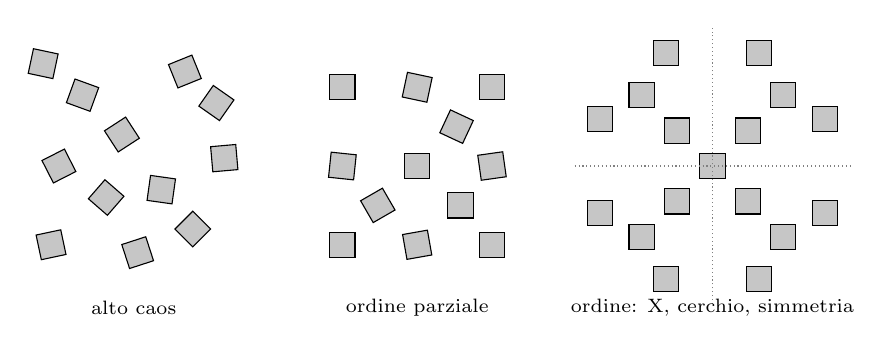
\begin{tikzpicture}[gd17cubo/.style={draw, fill=gray!45, minimum size=3.2mm,
  inner sep=0pt}]
  % caos
  \begin{scope}
    \foreach \x/\y/\r in {0.2/0.3/12, 1.1/1.7/33, 0.6/2.2/-20, 2.0/0.5/45,
      1.6/1.0/-8, 0.3/1.3/27, 2.3/2.1/-35, 1.3/0.2/18, 2.4/1.4/5, 0.9/0.9/-41,
      1.9/2.5/22, 0.1/2.6/-12}
      \node[gd17cubo, rotate=\r] at (\x,\y) {};
    \node[font=\scriptsize] at (1.25,-0.5) {alto caos};
  \end{scope}
  % intermedio
  \begin{scope}[xshift=3.6cm]
    \foreach \x/\y/\r in {0.3/0.3/0, 1.25/0.3/10, 2.2/0.3/0, 0.3/1.3/-6,
      1.25/1.3/0, 2.2/1.3/8, 0.3/2.3/0, 1.25/2.3/-12, 2.2/2.3/0, 0.75/0.8/30,
      1.75/1.8/-25, 1.8/0.8/0}
      \node[gd17cubo, rotate=\r] at (\x,\y) {};
    \node[font=\scriptsize] at (1.25,-0.5) {ordine parziale};
  \end{scope}
  % ordine: X + cerchio
  \begin{scope}[xshift=8.6cm, yshift=1.3cm]
    \foreach \d in {-0.9,-0.45,0.45,0.9}
      { \node[gd17cubo] at (\d,\d) {}; \node[gd17cubo] at (\d,-\d) {}; }
    \node[gd17cubo] at (0,0) {};
    \foreach \a in {0,45,...,315}
      \node[gd17cubo] at ({1.55*cos(\a+22.5)},{1.55*sin(\a+22.5)}) {};
    \draw[densely dotted, gray] (0,-1.75) -- (0,1.75);
    \draw[densely dotted, gray] (-1.75,0) -- (1.75,0);
    \node[font=\scriptsize] at (0,-1.8) {ordine: X, cerchio, simmetria};
  \end{scope}
\end{tikzpicture}
\caption{Ricostruzione dell'esercizio dei cubi. A destra, la composizione ordinata: una
X circondata da un cerchio, simmetrica su due assi; i cubi si contano contandone un
quarto e moltiplicando per quattro. Il numero e la disposizione dei cubi nelle slide
originali non sono noti: lo schema riproduce solo l'idea.}
\label{gd17:fig:cubi}
\end{figure}

\paragraph{La stanza simmetrica.} Lorenzo descrive un interno altamente
\textbf{simmetrico}: gli oggetti sono disposti in modo che, tracciata un'immaginaria
linea al centro dell'immagine, un lato si specchi nell'altro. Questo crea ``un
fortissimo senso di ordine'': appena si vede l'immagine si capisce subito dove ci si
trova, com'è disposta la stanza, che cosa fare per andare ad accendere la televisione.

\paragraph{La stanza caotica (e la domanda trappola).} A Francesco Muratore (``prendiamo
una persona a caso'') tocca una stanza piena di oggetti che si mischiano tra loro:
ordinata? ``Assolutamente no.'' E se dovesse trovare un percorso, dove andrebbe?
``Dovrei scavare attraverso gli oggetti.'' In realtà un percorso c'è, attorno a un
tavolino, dove resta uno spazio vuoto: ``era una domanda trappola, quindi non
preoccuparti''. Il punto è che in un ambiente a bassissimo ordine, quindi ad alto
caos, è impossibile orientarsi e avere una buona percezione dello spazio: ``c'è una
totale mancanza di struttura''. Il docente non vuole fare ``filosofia spicciola'' da
guru del self-help (``tenete in ordine l'ambiente e vivrete meglio''); ma è vero che
più un ambiente è caotico, più è difficile navigarlo, e più è difficile perfino
percepire com'è fatto.

\begin{definition}[Ordine]
Si parla di \textbf{ordine} quando si considera la \textbf{posizione} degli elementi
nello spazio e la \textbf{relazione} di questi elementi tra loro, organizzati in una
maniera che crea \textbf{sicurezza} in un individuo e lo aiuta a
\textbf{orientarsi}.
\end{definition}

\paragraph{L'ordine si sente d'istinto.} Già dalle prime domande si vede che tutti
hanno, d'istinto, una percezione degli spazi che si allinea con l'interior design, anche
senza saperla razionalizzare. Lo stesso vale per i giocatori: si accorgono dell'ordine
e del caos ``semplicemente per il fatto che da quando sono nati si trovano all'interno
di spazi del genere''. Al level designer serve sapere \emph{che cosa} rende uno spazio
ordinato o caotico per \textbf{connettersi a queste conoscenze istintive}, e per farlo
bisogna ``smembrare'' l'ordine nei suoi componenti.

\subsection{Le tre componenti dell'ordine}

L'ordine si può scomporre in \textbf{pattern}, \textbf{orientamento} e
\textbf{definizione degli spazi}, ciascuno con i suoi sotto-elementi
(figura~\ref{gd17:fig:mappa}). Il docente avverte che questa prima lezione del ciclo
tratta cose ``abbastanza istintive''.

\begin{figure}[ht]
\centering
\begin{tikzpicture}[
  gd17radice/.style={draw, rounded corners, fill=blue!15, font=\small\bfseries,
    minimum width=2.6cm, minimum height=7mm},
  gd17ramo/.style={draw, rounded corners, fill=blue!6, font=\small,
    minimum width=2.9cm, minimum height=6mm, align=center},
  gd17foglia/.style={draw, rounded corners, fill=white, font=\scriptsize,
    text width=2.5cm, align=center, minimum height=5mm},
  gd17freccia/.style={-{Stealth[length=2mm]}, thin}]
  \node[gd17radice] (room) at (0,0) {Room design};
  \node[gd17ramo] (ord) at (-4.2,-1.3) {\textbf{Order}\\(questa lezione)};
  \node[gd17ramo] (enr) at (0,-1.3) {Enrichment};
  \node[gd17ramo] (exp) at (4.2,-1.3) {Expression};
  \foreach \n in {ord,enr,exp} \draw[gd17freccia] (room) -- (\n);
  \node[gd17ramo, fill=green!8] (pat) at (-4.6,-3.0) {Pattern};
  \node[gd17ramo, fill=green!8] (ori) at (-0.9,-3.0) {Orientamento};
  \node[gd17ramo, fill=green!8] (spa) at (2.9,-3.0) {Definizione\\degli spazi};
  \foreach \n in {pat,ori,spa} \draw[gd17freccia] (ord.south) -- (\n.north);
  \node[gd17foglia] (p1) at (-4.6,-4.3) {di colori\\di forme};
  \node[gd17foglia] (p2) at (-4.6,-5.3) {creati da \emph{ricorrenza}\\e
    \emph{contrasto}};
  \node[gd17foglia] (o1) at (-0.9,-4.3) {identità (cultura)};
  \node[gd17foglia] (o2) at (-0.9,-5.0) {struttura (geografia)};
  \node[gd17foglia] (o3) at (-0.9,-5.7) {significato (persona)};
  \node[gd17foglia] (s1) at (2.9,-4.3) {enclosure};
  \node[gd17foglia] (s2) at (2.9,-5.2) {spazi espliciti\\e impliciti};
  \draw[gd17freccia] (pat) -- (p1); \draw[gd17freccia] (p1) -- (p2);
  \draw[gd17freccia] (ori) -- (o1); \draw[gd17freccia] (o1) -- (o2);
  \draw[gd17freccia] (o2) -- (o3);
  \draw[gd17freccia] (spa) -- (s1); \draw[gd17freccia] (s1) -- (s2);
\end{tikzpicture}
\caption{La mappa della lezione: il room design, i suoi tre macro fattori e le
componenti dell'ordine, con i sotto-elementi trattati nella lezione.}
\label{gd17:fig:mappa}
\end{figure}

% ---------------------------------------------------------------------
\section{Il pattern: colori e forme}
\label{gd17:sec:pattern}

\subsection{Una domanda preliminare e una definizione}

Prima di cominciare, una domanda importante: c'è qualcuno di
\textbf{daltonico},\footnote{Nella trascrizione ``dal tonico''.} o con una percezione
diversa dei colori? Il docente non vuole ripetere ciò che gli è successo una volta a
lezione: chiedere a una persona di descrivere i colori di una stanza e sentirsi
rispondere ``non ne sono così sicuro: sono daltonico, mi dispiace''. Nessuno: si parte.

L'elemento più riconoscibile dell'ordine è il \textbf{pattern}. Alberto ne dà una prima
definizione: ``una sequenza che viene ripetuta''; quindi la scala do, re, mi, fa, sol,
la, si, do è un pattern? ``Potrebbe esserlo. Dipende da come viene utilizzato.''

\begin{definition}[Pattern]
Un \textbf{pattern} è una sequenza di elementi ripetuti secondo un \textbf{ordine
logico} che è possibile notare.
\end{definition}

``Stavo per dire \emph{visivamente}'', ma i pattern possono essere di qualunque tipo,
anche sonori; e se i videogiochi si fruiscono soprattutto con gli occhi, ``ci sono
cose di design molto, molto fighe nell'ambito dei videogiochi che si usano solamente
con l'udito''. Ma non si divaga. Nella ricerca dell'ordine (``oggi parlerò molto come
un cavaliere Jedi: andiamo in cerca dell'ordine, facciamo di tutto per andare contro il
caos'') si riconoscono due tipi principali di pattern: i \textbf{pattern di colori} e
i \textbf{pattern di forme}.

Il docente porta allora ``metaforicamente alla lavagna'' ognuno degli studenti,
partendo ``dal basso verso l'alto, per una volta''. Le immagini sono fotografie di
interni; il capitolo le descrive attraverso ciò che ne dice la classe.

\subsection{Lorenzo: la stanza rossa e bianca}

\paragraph{Quadrati e alternanze.} Lorenzo nota quadrati ovunque e un'alternanza di
colori: il quadro a destra è un quadrato nel quadrato nel quadrato; il muro è un
rettangolo, davanti c'è un quadrato, il sofà è un quadrato con un quadrato disegnato
sotto. I colori si alternano dal pavimento verso il quadro: bianco, rosso, bianco,
rosso, grigio, rosso, bianco, rosso. Anche le finestre fanno un pattern (finestra,
sbarramento, finestra), con a loro volta un pattern interno di quadrati in alto, in basso
e rettangoli al centro, e la stessa \textbf{simmetria}, ``biassiale, su due assi, x e
y''. ``Non ci stiamo preoccupando della simmetria per adesso'': è un'immagine ``un po'
\emph{easy mode}'', perché estremamente strutturata.

\paragraph{La domanda trappola: quanti colori?} Lorenzo comincia a contare: il rosso, il
bianco, il grigio dietro al sofà, il verde della pianta, il nero; ``in realtà, visto che
la luce è una lunghezza d'onda, ti direi infiniti''; almeno quattro che saltano
all'occhio, almeno sei ben definiti. La risposta del docente:
\begin{quote}
Se vogliamo essere rigidamente stretti, ci sono \textbf{due colori} in questa immagine:
il bianco, il nero e il grigio, che varia dal bianco al nero, non sono considerati
colori, perché non hanno \emph{hue}, l'elemento del colore.
\end{quote}
È ``un vantaggio gigantesco'', anche per imparare a vestirsi: non avendo una tinta,
bianco, nero e grigio \textbf{stanno bene con qualunque colore}, ``sono il trucco per
come abbinare i colori''. Serve sempre un certo occhio, ma l'intera scala di grigi non
stona con nessuno dei due colori della stanza.\footnote{Il termine italiano che il
docente non ricorda è \emph{tinta} (o \emph{tonalità}): \emph{hue}, una delle tre
dimensioni del colore insieme a saturazione e luminosità. Bianco, nero e grigi sono i
colori \emph{acromatici}, privi di tinta. Lo stesso docente, più avanti, avverte di non
prendere ``esageratamente alla lettera'' queste nozioni: sono regole pratiche, non
teoria del colore rigorosa.}

\paragraph{Le piante negli angoli e il pizzico di caos.} Perché il verde compare solo in
un punto? Le piante sono tutte verticali, tendono verso l'alto, e sono messe nell'angolo
più in ombra, così come il vasetto nell'altro angolo: un pattern \textbf{piante negli
angoli}, studiato anche questo. Ma c'è di più: anche in un ambiente così rigidamente
ordinato c'è ``quel pizzichino di caos che ci aggiunge un po' di sapore''. Quella
``botta di colore verde'', non replicata altrove, \textbf{trattiene la stanza dal
sembrare completamente artificiale}.
\begin{quote}
E ora sapete perché esistono le piante nell'arredamento: aiutano molto a creare questa
sensazione di \textbf{spazio reale}.
\end{quote}

\subsection{Alberto: il bianco dominante e gli accenti azzurri}

\paragraph{L'alternanza.} Alberto nota l'azzurro e il bianco, \textbf{alternati}: nella
poltrona e nel poggiapiedi sono sullo stesso elemento (con un verde desaturato ``strano''),
mentre divano e tavolino ripetono l'alternanza su elementi diversi: cuscini azzurri su
un divano grigio, ``che è sempre tra il bianco e il nero''.

\paragraph{Dominante e accento.} Qual è il colore dominante? Quello che occupa più
spazio è probabilmente il bianco, ``ma a vista quello che prende attenzione è
l'azzurro''. Esattamente: uno spazio ``tra virgolette bianco'', fatto di sfumature di
bianco, con \textbf{accenti di blu}. Immerso in quello sfondo, il pattern degli
elementi blu ``spicca molto di più''. ``Anche questo è ordine, è studio degli interni.''

\paragraph{I ``bottoni''.} C'è anche un pattern creato da una lavorazione dei cuscini
(``mi viene da dire bottoni, ma non sono bottoni; chiedo scusa, non sono un sarto''),
ripetuta all'interno dello stesso cuscino e chiaramente studiata per cadere
perfettamente a metà del divano.\footnote{Dalla descrizione, con ogni probabilità la
lavorazione \emph{capitonné} (trapuntatura a bottoni). Il nome non compare nella
lezione.} ``È ovvio che se ti occupi di dettagli così esagerati c'hai un sacco di
soldi'', ma per chi se lo può permettere un lavoro studiato è un'ottima idea.

\paragraph{Rettangoli smussati.} Le forme prevalenti sono quadrati e rettangoli: i
cuscini, la poltrona, il poggiapiedi, la tovaglia sotto la pianta. Ma sono lo stesso tipo
di rettangoli dell'immagine precedente? No: qui gli angoli sono \textbf{tondeggianti}
per quasi tutti gli elementi, mentre nella stanza rossa e bianca erano geometricamente
netti, ``tanto che il divano non ci hanno neanche provato a farlo quadrato''.

\subsection{Francesco: il bagno verde, il legno e il meta-pattern}

\paragraph{Il pattern di materiale.} ``Qua le cose si fanno un po' più complesse.'' I
colori principali sono il verde e il bianco; ma a Francesco salta all'occhio il
pavimento in \textbf{legno} della doccia, che ritorna nella sedia in fondo a destra. E c'è
un terzo elemento in legno: la cornice del quadro. È un \textbf{pattern creato dai
materiali}: le tre cose sono studiate per stare insieme. ``Vi assicuro che se la doccia
avesse avuto un piatto in ceramica, non ci sarebbe stata tutta questa attenzione
all'utilizzo del legno in altri elementi dell'arredamento.''

\paragraph{Rettangoli.} I vetri della doccia, il muro interno della doccia (più
rettangolo che quadrato), le finestre, il quadro, gli asciugamani bianchi e neri appesi,
il muretto che divide la stanza, quello che sembra un cesto della biancheria (o uno
sgabello): tutto è costruito su rettangoli. L'unica eccezione è il lavabo al centro,
``una specie di lavapiedi''. C'è poi, di nuovo, una pianta a decorare il tavolino in
fondo.

\paragraph{Il soffitto e le piastrelle.} Guardando il soffitto, Francesco trova le
\textbf{travi a vista} (``popolari in certi tipi di case''; e qui ce ne sono di due
tipi) e le \textbf{piastrelle}, quadrate anche quelle, sulle pareti (``aiuto, non mi
ricordo come si chiamano'').\footnote{Nella trascrizione lo studente cerca la parola
(``le tegole, le travi?'', ``le piastre, le strette''): dal contesto si tratta delle
piastrelle della parete e delle travi del soffitto.} Colori tipici di un bagno, nota
lo studente; e il docente aggiunge la ragione pratica: dove esce l'acqua serve qualcosa
che non sia vernice e mattoni, ``altrimenti ti durano una settimana''.

\paragraph{Il meta-pattern.} ``Vogliamo esagerare?'' La stanza ha già ritmi molto
geometrici (le piastrelle, la pavimentazione non monocromatica); ma nell'arredamento è
stata fatta una scelta precisa sui \textbf{pattern di ornamento}, che si può vedere quasi
come un \textbf{meta-pattern}: \emph{ogni} elemento dell'arredo ha un pattern. La sedia
con i suoi elementi ``arzigogolati''; il tavolino, estremamente ricco di dettagli; il
mobiletto sotto, con buchi perfettamente simmetrici; un altro mobile con un decoro sulla
superficie.
\begin{quote}
Tutti i mobili di questa stanza hanno un pattern, e questo crea un pattern. Bellissimo!
Mi piace un sacco la poesia di questa cosa. È così che funziona l'attenzione ai dettagli
quando ti occupi di arredare le cose, o anche di vestirti, o di qualunque cosa, lato
estetico: c'è una struttura.
\end{quote}

\subsection{Antonino: il ciano, le forme circolari e il bilanciamento}

\paragraph{Lo sfondo non è il colore dominante.} Antonino indica il \textbf{ciano} come
colore dominante, e le forme circolari: un cerchio nero alla parete, le lampade, una
``testa'' a sinistra (una scultura); e un'alternanza tra il ciano e il bianco e il nero,
con stacchi bianchi o neri tra i mobili. Il docente lo corregge su due punti. Il ciano è
il colore che \emph{spicca} di più, non lo sfondo; e se si considerano dominanti, cioè
principali, elementi che in realtà sono messi in risalto da un contesto completamente
opposto, si legge male l'immagine. ``Bianco e nero non sono colori, ricordiamocelo'':
proprio per questo aiutano a far spiccare gli altri. (``Non entriamo nella teoria del
colore in maniera esagerata. Non sono un insegnante di arte: sono piccole nozioni che
uso per aiutarmi quando creo i miei spazi 3D.'')

\paragraph{Le forme regolari.} Quante figure geometriche regolari che non sono cerchi si
trovano? Le piastrelle esagonali; le gambe dei tavolini, che formano dei trapezi; i
cuscinetti delle poltrone, un po' ``bombati'' ma di base quadrati; la testa, fatta di
tanti poligoni; i triangolini sotto le lampade. E soprattutto le \textbf{pareti}: tanti
rettangoli e quadrati creati con dei rilievi. ``C'è un forte lavoro nel creare pattern
che si contrastano tra loro.''

\paragraph{Le simmetrie interne e il bilanciamento.} C'è anche un forte lavoro di
\textbf{simmetrie interne}. Un asse taglia a metà un focolare di design (``in una
posizione terribile, sinceramente, ma esteticamente molto bello''), il divano, e separa
le due lampade. Un'altra simmetria corre lungo la linea che divide la parete bianca da
quella nera, creando due pareti delle stesse dimensioni. Da un lato di questa linea c'è
la pianta, dall'altro la testa: non è una simmetria perfetta, ma \textbf{bilancia} il
lato con più elementi.
\begin{quote}
Se non ci fossero stati la pianta e la testa (e i vasi qua sotto), vista la presenza di
molti elementi in questo lato della stanza, l'altro lato avrebbe dato la percezione di
essere vuoto, che gli manca qualcosa. Per creare ordine, bisogna \textbf{metterci
qualcosa a compensare}.
\end{quote}

\subsection{Valerio: la stanza carica ma ordinata}

\paragraph{Tanti oggetti.} ``Ci buttiamo molto più sull'organico.'' La stanza di Valerio
si percepisce come più disordinata: molti oggetti, soprattutto al centro, ``molto più
appesantita di dettagli, molto più arricchita'' (``ci arriveremo in un'altra lezione,
all'enrichment''). Però ci sono delle forme: un quadrato al centro dentro un rettangolo
con i due divani, il tavolino, le due librerie, la finestra, la porta.

\paragraph{Lasciamo stare i rettangoli.} ``È inevitabile che nella stragrande maggioranza
degli spazi interni i quadrati, barra rettangoli, siano uno dei pattern principali'':
pareti, porte e finestre sono rettangoli, e l'arredo continua un pattern che c'è già.
Punto. Ma quali pattern non sono fatti di rettangoli? Le piante, tutte al centro; e i
\textbf{cuscini} dei divani: ``sono presenti lo stesso numero di cuscini con le stesse
tonalità cromatiche'' (il docente chiede una descrizione precisa, e la ottiene). E poi
una ``bellissima osservazione'': nella parte bassa della foto i colori tendono allo
\textbf{scuro}, in quella alta al \textbf{chiaro}. ``Occhio, mi piace.''

\paragraph{Il blu delle tende.} Il docente accelera (``abbiamo un sacco di roba da
vedere''). Le tende di un azzurro così acceso, normalmente, ``fanno un po' kitsch, un po'
brutto''; qui sono bilanciate dal resto della stanza, dove blu e azzurro sono già usati
come accenti nei cuscini, nel pavimento e nei fiori. ``C'è un motivo se al centro non sono
state messe delle rose'': la palette gioca attorno al blu, al verde e a un marrone chiaro
che in alcuni punti è quasi giallo.

\paragraph{Carica, ma non caotica.} Nonostante sia ``strapiena di dettagli, di
soprammobili, di piante'', questa stanza non ha lo stesso effetto della stanza caotica
vista prima (sezione~\ref{gd17:sec:ordine}): ``spero che la differenza sia molto, molto
evidente, nonostante entrambe siano stracariche di roba''. La quantità di oggetti non
determina il caos: lo determina l'assenza di pattern.

\subsection{Francesca: la sala studio e le forme complesse}

\paragraph{Due famiglie di forme.} Francesca vede rettangoli su tutte le superfici che
chiudono la stanza (pareti, soffitto, pavimento), ognuna con una texture ripetuta; sulla
parete in fondo a destra, delle mezze sfere, delle ``lune'', che riprendono
l'arredamento centrale: i \textbf{pendenti}, figure bombate e allungate che giocano sulla
verticalità e sulle forme smussate, e che ritornano nell'ampolla sul tavolo e nelle gambe
del tavolo, morbide anche quelle. Le sedie, invece, hanno pattern più geometrici, che
riprendono la parete di mattoni e il pavimento, con piastrelle ``un po' a forma di
frecce''.\footnote{Con ogni probabilità un parquet o un pavimento a spina di pesce; la
trascrizione (``parche'') non permette di dirlo con certezza.}
\begin{quote}
Questa è una cosa importantissima da notare: quando si parla di pattern, non si parla
solo di ripetizione di geometrie semplici come rettangoli, triangoli, cerchi. Possono
essere anche \textbf{geometrie complesse} come queste che, se sono ripetute con una
certa intenzione, creano effettivamente un pattern.
\end{quote}

\paragraph{I colori del legno e dei libri.} I colori vanno tutti sul marrone, con
tonalità calde: chiari nelle pagine dei libri, negli interni delle sedie, sul muro, sul
soffitto (più verso il panna, che riprende la trasparenza dell'arredo centrale) e sul
pavimento; scuri nei bordi di quasi tutto, tavolo e mobili compresi. ``Rosso, arancione e
marrone sono in realtà variazioni dello stesso colore.''\footnote{Il docente aggiunge che
il marrone, ``a livello di teoria del colore'', è un po' ``un rosso molto scuro''. Più
precisamente il marrone è una tinta arancione-rossa a bassa luminosità e saturazione: la
sostanza dell'osservazione (rosso, arancione e marrone appartengono alla stessa famiglia
calda) resta corretta.} Le due piante a sinistra, verdi, riprendono il panorama
esterno: c'è un parallelo tra le piantine dentro e gli alberi fuori. Anche le copertine
dei libri vanno verso colori ``legnosi''.
\begin{quote}
È un ambiente pensato per quello che c'è al centro della stanza: riprende le forme e i
colori dei libri. C'è uno studio molto forte per renderlo \textbf{armonioso} non solo
con se stesso, ma anche con la cosa che lo occupa e con l'ambiente esterno.
\end{quote}
Potrebbe essere la sala studio di una biblioteca ``di altissimo livello, di quelle con
volumi proprio rari''.

\subsection{La carrellata: la simmetria di bilanciamento e l'aereo di lusso}

Per non ripetere tutto con gli altri, il docente scorre velocemente le immagini restanti.

\paragraph{La simmetria di bilanciamento.} Un esempio ``fortissimo di simmetria'', che
riprende quanto emerso con la testa e la pianta: una \textbf{simmetria di bilanciamento}
tra elementi che non sono gli stessi, ma che \textbf{svolgono visivamente la stessa
funzione}. L'elemento di destra è stato appoggiato sopra dei libri proprio per avere la
stessa altezza di quello di sinistra e bilanciare la composizione. ``Questa è un'altra
cosa su cui iniziare a riflettere: la composizione.''

\paragraph{Bianco, nero e luce colorata.} Un ambiente totalmente bianco, in cui l'unico
vero colore viene dalle luci (``un effetto molto fantascientifico''), e un mobilio diviso
per funzione: bianchi o grigio chiaro i mobili su cui appoggiare sé stessi o qualcosa,
\textbf{neri} gli oggetti funzionali (le casse, le luci, la televisione).

\paragraph{Forme affusolate e rettangolari.} In un altro interno, i contenitori d'acqua
hanno forme affusolate, mentre il mobilio è rettangolare.

\paragraph{L'aereo di lusso.} E per finire ``le cose un po' più avanzate'': l'interno di
un aereo di ultralusso, vincitore di un premio internazionale di design nel
2016,\footnote{Nella trascrizione ``International IOT and Aviation Awards del 2016'':
quasi certamente gli \emph{International Yacht \& Aviation Awards}, premi di design per
interni di yacht e aerei. L'aereo non è nominato.} che ``fa dello studio di pattern una
roba quasi scientifica''. Si rifiuta ogni angolo: tutto è ammorbidito, il tavolino ha gli
angoli tondi, i mobiletti hanno forme affusolate, ``anche se stai sacrificando molto
spazio''. Hanno creato ``un salotto volante''. E i pannelli rettangolari affusolati del
soffitto sono stati disegnati per \textbf{richiamare i pannelli tipici di un aeroplano},
il cui interno è costruito in un modo molto particolare, di cui chi ha progettato questo
interior design ha tenuto conto. ``Tutte queste cose noi le possiamo usare nella nostra
disciplina.''

\paragraph{La pausa.} Quindici minuti di pausa: ``ci vediamo tra le 45 e le 50''.

\paragraph{Approfondimento: dai pattern di Alexander a The Sims.} Il termine
\emph{pattern} ha in architettura un'eco precisa: \emph{A Pattern Language} di
Christopher Alexander (con Sara Ishikawa e Murray Silverstein), un catalogo di soluzioni
spaziali ricorrenti, dalle città alle stanze, che Totten consiglia a chi vuole
organizzare uno spazio. In una nota, Totten ricorda un aneddoto noto: Will Wright fu
ispirato a creare \emph{The Sims} proprio dalla lettura di \emph{A Pattern Language};
il gioco nacque come un gioco di costruzione di spazi secondo il linguaggio di pattern di
Alexander, e i Sims, in origine, servivano a ``valutare'' l'uso dei pattern da parte del
giocatore. I pattern della lezione sono più elementari (colori e forme), ma l'idea è la
stessa: uno spazio piacevole è uno spazio in cui le soluzioni ricorrono in modo
riconoscibile.

% ---------------------------------------------------------------------
\section{Ricorrenza e contrasto}
\label{gd17:sec:ricorrenza}

Si riprende ``a raffica'', in ordine inverso, partendo da Francesca. Per analizzare i
pattern un po' più in profondità, il docente introduce \textbf{due elementi che aiutano a
crearli}:
\begin{description}
  \item[Ricorrenza:] \emph{quanto spesso} ricorre un certo elemento, o una certa
        struttura di elementi.
  \item[Contrasto:] \emph{che cosa} rende questi elementi qualcosa che
        \textbf{spicca} rispetto a ciò che li circonda.
\end{description}

\begin{figure}[ht]
\centering
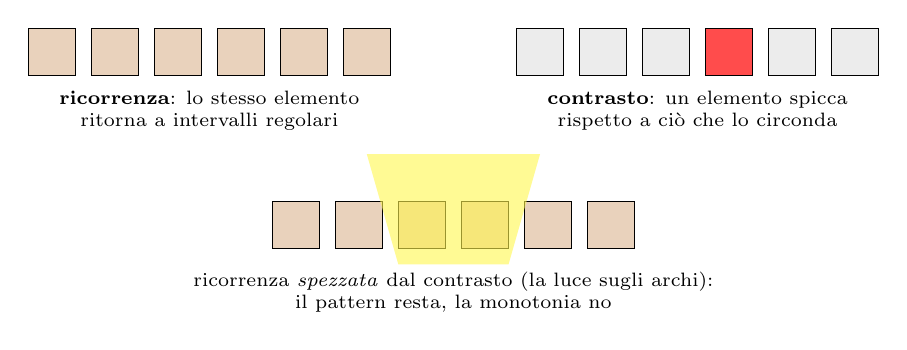
\begin{tikzpicture}[gd17q/.style={draw, minimum size=6mm, inner sep=0pt}]
  % ricorrenza
  \begin{scope}
    \foreach \i in {0,...,5} \node[gd17q, fill=brown!35] at (\i*0.8,0) {};
    \node[font=\scriptsize, align=center] at (2,-0.75)
      {\textbf{ricorrenza}: lo stesso elemento\\ritorna a intervalli regolari};
  \end{scope}
  % contrasto
  \begin{scope}[xshift=6.2cm]
    \foreach \i in {0,...,5} \node[gd17q, fill=gray!15] at (\i*0.8,0) {};
    \node[gd17q, fill=red!70] at (2.4,0) {};
    \node[font=\scriptsize, align=center] at (2,-0.75)
      {\textbf{contrasto}: un elemento spicca\\rispetto a ciò che lo circonda};
  \end{scope}
  % ripetizione spezzata
  \begin{scope}[yshift=-2.2cm, xshift=3.1cm]
    \foreach \i in {0,...,5} \node[gd17q, fill=brown!35] at (\i*0.8,0) {};
    \fill[yellow!70, opacity=0.6] (1.3,-0.5) -- (2.7,-0.5) -- (3.1,0.9) -- (0.9,0.9)
      -- cycle;
    \node[font=\scriptsize, align=center] at (2,-0.85)
      {ricorrenza \emph{spezzata} dal contrasto (la luce sugli archi):\\
       il pattern resta, la monotonia no};
  \end{scope}
\end{tikzpicture}
\caption{Ricorrenza e contrasto, schematicamente. La terza riga anticipa l'esempio degli
archi (sezione~\ref{gd17:sec:archi}): un elemento che varia la ripetizione senza
distruggerla.}
\label{gd17:fig:ricorrenza}
\end{figure}

\subsection{Francesca: il bianco e il legno}

Francesca descrive un ambiente dai colori chiari, ``morbidi'', con un \textbf{contrasto
netto}: pareti e pavimento prettamente bianchi, mentre travi, scale, porte e cassetti sono
in \textbf{legno}. ``Attenzione, qua c'è una cosa interessante: c'è un pattern che si crea
dalla scelta del materiale.'' Tutto ciò che non è muro, soffitto o pavimento è in legno,
dalla trave più grezza in alto a destra al parquet accanto alla porta; più chiaro
all'esterno, più scuro all'interno (i cassetti, la porta, più chiara in alto e con
venature più scure in basso, ``anche per questioni di come sono illuminati'', ma è
giusto). La ricorrenza è sempre questa: bianco o chiaro, ma in legno.

Le forme sono tutte geometriche, righe nette, con tre eccezioni: l'\textbf{oblò} sulla
porta a destra, gli \textbf{archetti} sulle mensoline a sinistra e una
\textbf{lampada} circolare. Il docente nota l'intenzione: le linee tondeggianti sono tutte
elementi \textbf{verticali}, che pendono o sono attaccati alle pareti. ``C'è sempre un
pattern.'' E, per chiudere, un ``pesantissimo'' pattern di quadrati: i cassetti ricavati
in un lato della scala.

\subsection{Valerio: gli zaini e le due pareti}

\paragraph{Contrasto e gradiente.} Gli zaini e le borse appesi alla parete sono messi in
risalto da uno \textbf{sfondo bianco} rispetto al resto, scuro: ``un contrasto, esatto''.
E i colori degli zaini ``sono ordinati'', molto simili tra loro: ``stanno creando un
gradiente'', ``questa è teoria del colore, ma ottima osservazione anche quella''. Sotto,
degli scaffali che non hanno lo stesso numero di elementi, ma su cui gli oggetti seguono
\textbf{la stessa struttura}: un pattern ``come quelli visti in precedenza'', che non usa
le stesse identiche cose, ma la stessa struttura di elementi. Sulla parete c'è anche
un'immagine (non una finestra né uno schermo: ``una specie di murale''), più chiara, e
una pianta che contrasta con lo sfondo neutro.

\paragraph{Lo stesso schema su due pareti.} Il docente chiede di mettere in relazione la
fotografia appesa con la parete degli zaini, ``come elementi all'interno della
composizione''. C'è un pattern creato quasi da due soli elementi: una \textbf{parete
completamente nera} con un \textbf{rettangolo bianco-crema} che ne occupa lo spazio, e lo
stesso schema ripetuto sull'altra parete. Pur con dimensioni diverse, ``sono lo stesso
elemento ripetuto su due pareti diverse. Non è perfetta simmetria, ma è lo stesso schema,
è la stessa ripetizione.''

\subsection{Antonino: i cassetti e gli accenti rossi}

\paragraph{Il cassetto come elemento ripetuto.} Antonino nota il contrasto tra la
struttura nera del letto (``più un marrone scurissimo, sinceramente, ma qua stiamo a
cercare il pelo nell'uovo'') e la parete bianca e verde chiaro, oltre al legno chiaro.
Che cosa si ripete? Antonino vede i gradini, identici; il docente lo invita a vederli come
\textbf{cassetti}: cinque nella scala e quattro nella base del letto.
\begin{quote}
Qui il cassetto diventa un elemento ripetitivo che \textbf{tiene insieme}, nella sua
ripetizione, la parte sinistra della scala e la parte centrale del letto. Questo è un
pattern molto, molto palese.
\end{quote}
Anche i cuscini riprendono i colori usati, con un rosso che ``spezza''; il tappeto si
abbina al legno e al materasso. ``C'è sempre una struttura di ripetizione dei colori: pochi
elementi ripetuti e occasionalmente qualche accento.''

\paragraph{Quando le piante non bastano.} Qui gli \textbf{accenti}, le piccole parti di
colore che spiccano, non sono dati dalle piante, come in molte foto precedenti: con una
parete verde così grande, il verde delle piante non spicca come spiccava nella sala
marrone e bianca di Francesca. Si è scelto allora di mettere accenti \textbf{rossi}, che,
non comparendo altrove, spiccano di più. Rosso e verde sono \textbf{colori
complementari}, ``sono anche i colori del Natale, motivo per cui non sono usati
tantissimo nel design, perché suggeriscono il Natale''.\footnote{Rosso e verde sono
complementari nel modello tradizionale dei pittori (rosso, giallo, blu). Nel modello
additivo RGB, quello degli schermi e quindi dei motori di gioco, il complementare del
rosso è il ciano, e quello del verde il magenta. Il docente stesso rimanda
l'approfondimento dei complementari a chi è interessato.}

\subsection{Francesco: gli archi e la luce che spezza la ripetizione}
\label{gd17:sec:archi}

``Questa è bella, abbastanza facile.'' Francesco vede una grande ripetizione di
\textbf{archi}, praticamente tutti uguali, con gli stessi colori; colonne fatte allo
stesso modo; un lampadario quasi in ogni campata. Fatica però a trovare un contrasto, se
non la luce che entra dall'alto.

Ed è proprio quello il punto. La luce entra da un'apertura centrale e da navate laterali
più strette, e non illumina tutto allo stesso modo.
\begin{quote}
In un ambiente creato da un pattern incredibilmente regolare, che quindi rischierebbe di
essere molto ripetitivo (e bisogna fare attenzione a non creare un'esagerata ripetitività
quando si creano questi pattern), queste differenze di luce ci permettono di avere
\textbf{contrasto e varietà} che spezzano la ripetitività del pattern. È questo il
trucco che si usa per far funzionare ambienti estremamente ripetitivi: trovare qualcosa
che permetta di avere la ripetizione, ma che visivamente non sia sempre uguale.
\end{quote}
Il luogo esiste davvero, ``ma non chiedetemi come si chiama, perché non me lo
ricordo''.\footnote{Il luogo non è identificabile dalla registrazione.}

\subsection{Alberto: la cucina dei gatti}

``Spero ti piacciano i gatti.'' Le foto sono piene di gatti, ``ma non credo che possiamo
considerarli parte dell'arredamento''. Alberto nota il colore del legno ricorrente in
tutto l'arredo: il tavolo dell'isola, i cassetti e le ante della cucina hanno lo stesso
colore. Le tende ripetono un altro colore, diverso da quello di mobili e pareti (Alberto
le vede grigie: ``credo sia più una questione di illuminazione''). Le piante dentro
riprendono le piante fuori; moltissimi rettangoli, moltissime finestre: ``un ambiente
super illuminato. Probabilmente questa casa è un incubo da riscaldare, sarò sincero''. E
di nuovo una pianta in ogni stanza per creare un piccolo contrasto: ``in un ambiente in
cui i gatti girano così liberamente, lo trovo estremamente rischioso. Infatti questo
gatto qua sta già avendo delle idee''.

\subsection{Lorenzo: la cucina blu e rossa}

\paragraph{Le aree e i materiali.} Ultimo, Lorenzo, su una cucina dai colori fortissimi.
Si vedono \textbf{aree ben definite, porzionate dal colore}, e molto contrasto di
materiale. Il legno ricorre: in primissimo piano, nello scaffale di destra (quello senza
decori floreali), in fondo sulla cucina. Ricorrono anche le \textbf{decorazioni
floreali}: nelle tende, nello scaffale di sinistra con i piatti; e richiamano la
\textbf{pianta} in alto. Senza quella pianta, osserva Lorenzo, lo spazio potrebbe dare un
senso di vuoto.\footnote{Nella trascrizione: ``sembrerebbe quasi una bekter''. La parola
non è ricostruibile.}
\begin{quote}
Le piante servono a questo: a creare un ambiente che sembra meno artificiale, che non ti
dà quella sensazione \textbf{liminale} di uno spazio totalmente finto. Le piante
ravvivano gli ambienti.
\end{quote}
Lorenzo nota anche il telefono a muro, in una posizione insolita (ma le sedie sono basse
rispetto agli scaffali, quindi ci sta), e il mobiletto in primo piano, molto grosso in
prospettiva.

\paragraph{I colori protagonisti.} Il pavimento rosso, molto lucido, riflette le sedie
``quasi color lava''. Blu, legno e rosso si sposano bene, soprattutto il blu e il rosso;
e fuori dalla finestra c'è un blu (forse la foto è stata scattata al crepuscolo) che
richiama la cucina. Luci dall'alto sulla cucina e sul tavolo dove si mangia, ``un classico
per illuminare bene la parte centrale della stanza''. Rispetto a quasi tutti gli ambienti
precedenti, qui i colori ``sono proprio protagonisti'', molto saturi, ``che picchiano
forte''.

\paragraph{Bella, ma vivibile?} La troveresti brutta? Lorenzo la troverebbe gradevole da
visitare, come la stanza-museo di un designer, ma ``forse non vivibile''; eppure il
condizionatore, il citofono e il telefono dicono che qualcuno ci vive davvero. ``Non è
nelle mie corde'', ma ci potrebbe vivere qualche personaggio eccentrico.\footnote{Nella
trascrizione: ``Com'è che si chiama il Gioioio? Ma il Gioioio ci vive''. Il personaggio
citato non è ricostruibile.} Il docente capisce: chi arreda così è una persona molto
eccentrica. Ma usa spesso questa foto per un motivo:
\begin{quote}
Non si deve per forza utilizzare bianco, nero, beige, crema e basta nell'arredamento degli
ambienti. Se vuoi spingerti, puoi spingerti. Serve \textbf{cognizione di causa} e un po' di
studio per farli funzionare, invece di farli sembrare una cosa pacchiana. Questo, secondo
me, è uno di quegli ambienti che funzionano.
\end{quote}
L'angolo cottura è dedicato al \textbf{blu}, l'angolo sala da pranzo al \textbf{rosso}:
una \textbf{divisione degli spazi} (un'altra cosa che si vedrà); e il \textbf{legno} (il
tavolo, gli scaffali) fa da \textbf{elemento di continuità} tra zone dai colori dominanti
molto diversi. Al docente la casa piace parecchio, ``però magari abitarci potrebbe essere
un po' pesante'': di solito la tendenza è di stare il più neutri possibile.

\paragraph{Il tema.} Un'ultima nota di Lorenzo: le sedie hanno tutte un pattern molto
specifico, \textbf{vermicolare},\footnote{Nella trascrizione ``verniculare'': un motivo
a linee sinuose simili a vermi, qui vicino al floreale. Lo studente lo paragona anche a dei
mitocondri.} non floreale ma molto vicino, che si ricollega alla pianta in alto a destra.
Il docente generalizza:
\begin{quote}
Chi ha fatto il design di questo ambiente ha scelto un \textbf{tema} che fa da
\textbf{filo conduttore} per gli elementi dell'ambiente, per tirare insieme l'intera
struttura. Sono cose molto difficili, molto complesse da fare.
\end{quote}

\subsection{La baita e la stanza RGB}

\paragraph{La baita.} Lo si vede ancora più chiaramente nelle baite e negli edifici più
antichi. L'esempio è un render (``chiaramente non è una fotografia''): colori tutti
tendenti al marrone, caldi, ``confortevoli''; travi che creano un ritmo sopra; un
lampadario a gocce che crea un altro pattern. E un \textbf{elemento di continuità tra
interno ed esterno}: le pietre che rivestono il camino (``ricchezza enorme avere il camino
nel bagno, adoro'', nell'angolo bagno della stanza) proseguono quasi direttamente verso il
balcone, facendo da congiunzione tra i due ambienti.

\paragraph{La stanza RGB.} In un altro ambiente i colori si dividono per zone: rosso-rosa
al centro, blu a destra (dalla finestra), verde a sinistra: ``rosso, verde, blu, RGB,
battuta da computer''. Ma c'è sempre un certo livello di struttura.

\subsection{La regola delle regole interne}

Il messaggio che il docente vuole far passare è questo:
\begin{quote}
Qualunque cosa voi facciate quando organizzate uno spazio, l'importante è \textbf{darvi
delle regole interne da seguire}. Darvi un filo conduttore, un'idea, un tema; cercare dei
pattern che potete usare per creare ordine. Non deve essere, ripetiamolo ancora una volta,
la perfezione della ripetizione geometrica simmetrica: deve essere qualcosa a cui il
cervello umano si può aggrappare per dire istintivamente: riconosco che c'è un certo ordine
nella scelta di come è stato creato questo ambiente.
\end{quote}
Vale anche per zone piccolissime, ``anche per un semplice angolo di una stanza'': se si
vuole creare qualcosa di visivamente piacevole, in cui sia un piacere, ``quasi a livello di
percezione fisica'', passare del tempo, il trucco è trovare ciò che gli dà ordine: pattern,
colori, contrasto. ``Queste cose le applicheremo poi al mondo dei videogiochi.''

\subsection{Un videogioco: la concept art di Horizon Zero Dawn}

Ed ecco il primo videogioco: una \textbf{concept art} di \emph{Horizon Zero Dawn}. Che
pattern ci sono? Si offre una volontaria.

\paragraph{I pattern di luce.} Le luci che entrano da destra sembrano ``quasi
caravaggesche'' (``ci dedicheremo un po' di tempo quando parleremo di nuovo di luci''), e
l'azzurro scuro ``è un classico''. Quali sono i pattern di luce? Da tutte le fenditure
entrano luci molto oblique, in linea dritta. La studentessa prova a dire quali sono
direzionali e quale sembra una point light, ma il docente la ferma:
\begin{quote}
Non concentriamoci su che cosa potrebbe star succedendo dietro le quinte.
\textbf{Descriviamo l'intenzione, l'effetto, non il nome.}
\end{quote}
È un'indicazione di metodo: in una concept art non ci sono ``luci di Unreal'', ci sono
scelte visive.

\paragraph{Le forme cristalline.} Gli elementi ``cristallini'' (``non so esattamente cosa
siano, sarò sincero'') creano un pattern di forme oblique, non sempre orientate nella
stessa direzione: a volte verso destra, a volte verso sinistra. La formazione in basso a
sinistra ha una gemella \textbf{speculare} a destra, separata al centro dalla fenditura di
luce.\footnote{La trascrizione cita anche ``Horizon Zero 2'': potrebbe trattarsi di una
seconda immagine o del seguito (\emph{Horizon Forbidden West}), ma non è ricostruibile.
Non è chiaro neppure che cosa siano gli elementi ``cristallini'' della concept art.}

\paragraph{Il contrasto.} I colori sono molto scuri, tendenti al blu scuro, quasi nero; ma
ci sono punti illuminati fortissimamente. Il docente chiede quale sia il rapporto fra il
punto più luminoso e quello meno luminoso della foto, ma non vuole parlare di luminosità
in senso tecnico: la parola è \textbf{contrasto}. È un ambiente scuro con punti illuminati
molto fortemente; e il contrasto si può creare con qualunque cosa, con la luce come con i
colori. La luce mette in evidenza gli oggetti \textbf{metallici} (``la luce è la cosa che
ci permette di distinguere gli elementi metallici''); i cavi che sporgono dagli elementi
più tecnologici sulle pareti, e i lampi di energia che fanno ``sprazzi'' negli spazi bui e
ricordano i cavi, creano un'altra ripetizione.
\begin{quote}
Ci sono pattern anche in questa immagine, che a colpo d'occhio sembra non avere una
struttura. Ma una struttura ce l'ha, e se ci fate attenzione una struttura la trovate
ovunque, in ogni cosa.
\end{quote}

\paragraph{Approfondimento: i pattern che insegnano.} Totten mostra come i pattern abbiano
nei livelli anche una funzione \emph{comunicativa}. Uno spazio ripetuto con regolarità (la
stanza di salvataggio prima del boss, il corridoio che annuncia l'arena) addestra il
giocatore a riconoscerlo e a prevedere che cosa verrà; e un simbolo ripetuto
nell'ambiente, come il lambda della resistenza in \emph{Half-Life 2}, posto vicino ai
depositi di oggetti utili o alle pause nell'azione, finisce per significare ``qui c'è
qualcosa di buono'' senza bisogno di spiegazioni. È la ricorrenza della lezione spostata
dal piano estetico a quello del gameplay: un pattern riconoscibile non solo ordina lo
spazio, ma \textbf{insegna}.

% ---------------------------------------------------------------------
\section{L'orientamento: identità, struttura, significato}
\label{gd17:sec:orientamento}

\begin{definition}[Orientamento]
L'\textbf{orientamento} è la capacità, o la possibilità che si dà a una persona che si
trova in uno spazio (o che lo osserva), di capire qual è la sua \textbf{posizione
relativa} rispetto agli altri oggetti, o la posizione relativa degli oggetti tra loro: la
capacità di orientarsi all'interno di uno spazio.
\end{definition}

Non si tratta di sapere dove sono il nord e il sud, avverte il docente più avanti, ma di
capire dove ci si trova e in che tipo di spazio. Questa capacità è data da \textbf{tre
tipi di elementi}: l'\textbf{identità}, la \textbf{struttura} e il
\textbf{significato}. ``E qui le cose si iniziano a fare veramente interessanti.''

\subsection{L'identità}

\paragraph{La chiesa romanica.} ``Che cos'è questo edificio?'' Per Antonino è una
\textbf{chiesa}: lo dicono il tetto e il campanile. Dove si trova? In città; ma in che
paese, Finlandia, Palermo, Stati Uniti? Antonino guarda le targhe delle auto
(``europee'') e il docente lo ferma: ``così stai imbrogliando''. Guardando la chiesa,
Lorenzo nota gli \textbf{archetti} dello stile \textbf{romanico}, la torre campanaria, e
propone il nord Italia.\footnote{Lo studente colloca lo stile romanico attorno al 1400,
correggendosi da solo (``non mi ricordo esattamente''): in realtà il romanico è lo stile
dei secoli XI--XII (in Italia fino all'inizio del XIII); nel 1400 si è già nel gotico
tardo e nel primo Rinascimento.} Il docente concorda: nord Italia, se non Milano, la
pianura padana, perché questo era l'aspetto tipico delle chiese di quella zona; in centro
a Milano se ne vedono tantissime. Uno studente ne ricorda una simile davanti a una fermata
della metropolitana (``Conciliazione?'', ``no, scherzo'').
\begin{quote}
Questa è l'\textbf{identità}: la capacità di riconoscere in uno spazio, in un'immagine,
elementi che ci permettono di identificare quello che stiamo guardando. È la cosa che ci
permette di rispondere automaticamente alla domanda: \emph{questo che cos'è?}
\end{quote}
È un argomento che tornerà l'anno prossimo da un altro punto di vista, quello delle
\textbf{affordance} (anche \emph{culturali}), importantissime nel design degli elementi
interattivi; per ora lo si tiene come elemento di interior design.

\paragraph{I mulini.} Ad Alberto tocca un'immagine di mulini (``dei mulini\ldots{} punto
di domanda?''). Mulini a vento, ma non ``come quelli che trovi sulle Alpi''. In che paese
siamo? ``Non ne ho la minima idea. Sicilia?'' Il docente propone le opzioni: Sicilia, Nord
Africa, Cina, Danimarca, Olanda? ``Nord Europa, secondo me.'' Olanda o Danimarca,
probabilmente: paesi che \textbf{culturalmente} hanno questo tipo di edifici. È la
\textbf{componente culturale} del lavoro sull'ordine: elementi culturali orientano la
nostra percezione degli spazi; se quei mulini non fossero stati a vento, si sarebbe
percepito lo spazio in un altro modo.

\paragraph{La sagrestia.} A Francesca: dove ci troviamo? ``Italia sicuramente'', o un paese
europeo non laico, perché c'è un \textbf{crocifisso}. Ma la domanda era: \emph{in che
edificio}? Una chiesa, un edificio pubblico (un notaio, un'aula scolastica), forse
l'ufficio di una scuola di suore. Il docente, ``da persona che per un certo periodo della
sua vita ha frequentato ambienti molto cattolici'', è sicuro che anche senza il crocifisso,
dallo stile dei mobili e delle sedie, avrebbe detto: \textbf{una sagrestia}, o l'ufficio
di un prete; un ambiente ``non solo cristiano, proprio cattolico''.

\paragraph{Le identità non sono universali.} Ed ecco l'avvertenza, su cui si tornerà:
\textbf{gli elementi culturali non sono necessariamente condivisi da tutti}. Una persona
cresciuta, ``mettiamo un posto a caso'', a Tokyo, magari non avrebbe avuto la stessa
connessione immediata con quell'ambiente. È uno dei motivi per cui negli anime si vedono
spesso croci o suore usate ``senza una vera cognizione'' della religiosità
cattolico-cristiana: elementi scardinati dal loro contesto culturale.

\subsection{La struttura}

A volte non servono elementi architettonici o di arredamento a cui ``aggrapparsi'': basta
la \textbf{sola struttura} a dire in che tipo di spazio ci si trova.

\paragraph{Il centro commerciale.} Francesco, davanti a un grande interno, pensa prima allo
spazio aperto di una nave da crociera, poi a un \textbf{centro commerciale}: per i negozi,
ma anche per ``la forma in sé''. I centri commerciali hanno tutti più o meno la stessa
struttura: uno \textbf{spazio vuoto centrale distribuito su più piani}, con una fonte di
luce dall'alto per tutto il luogo. Il perché è commerciale: da dovunque ci si trovi si
vedono tutti gli altri negozi, ``ah, c'è Uniqlo al secondo piano, facciamo un
salto'',\footnote{Nella trascrizione ``Unicro''.} ``oh, c'è un negozio Apple, vediamo se
hanno qualche accessorio''. ``È fatto apposta per darti un'esperienza di shopping che ti
attiri dovunque ti trovi.''

\paragraph{Senza le insegne.} E se si togliessero i nomi dei negozi? Francesco direbbe
forse una nave da crociera; ed è possibile, perché le crociere sono studiate per simulare
proprio quell'esperienza. Ma tra un \textbf{complesso di appartamenti} e un centro
commerciale? Centro commerciale, per le forme. Risposta giusta, anche se la struttura con
lo spazio aperto centrale e i piani che si guardano esiste anche in certi complessi
residenziali, come le \textbf{Vele di Scampia}. La differenza fondamentale sono le
\textbf{vetrine}: in un condominio ci sarebbero porte e, più ancora, tende, qualcosa che
impedisca a chiunque passi di vedere che cosa c'è in casa.
\begin{quote}
Questa è la \textbf{struttura}: la disposizione dello spazio che permette a chi lo occupa
di sapersi orientare, di capire dove si trova.
\end{quote}

\paragraph{Il vicolo europeo.} A Lorenzo tocca un vicolo con un'osteria. Genova? Il
docente pensa di no: Genova è stretta tra il mare e le montagne, ``molto verticale'', ``è
praticamente impossibile vedere l'orizzonte senza vedere o il mare o un muro di edifici che
si sporgono verso l'alto''; ``molto claustrofobica'', almeno nella sua impressione. Non
interessa la città, però: in che \textbf{continente} siamo? Europa. E se le case fossero
fatte solo di forme, senza muri scrostati, finestre e grondaie? Lorenzo direbbe comunque
Europa: piano terra, primo, secondo piano; ``dubito che riesca a trovare un edificio del
genere'' negli Stati Uniti. Il docente scommette su \textbf{Roma}, per la pavimentazione,
il colore delle pareti e la passione romana per le piante rampicanti. E conferma il
ragionamento:
\begin{quote}
Anche se fossero solo giganteschi cubi e tetti, c'è qualcosa che ci dice che questa è
l'Europa: palazzi di due, tre, massimo quattro piani e strade strette, tipici delle
vecchie città di origine medievale o rinascimentale. Negli Stati Uniti, costruiti molto
più recentemente, le città sono basate sulle misure delle \textbf{automobili}, non di
persone e cavalli: le strade sono molto più larghe. La sola struttura ci suggerisce
elementi di identità, ci comunica dove ci troviamo.
\end{quote}
A uno studente il vicolo ricorda la sua città, Sassari: vicoli stretti, piccoli. ``Tutte
città di vecchia data, molto romantiche, molto medievali, se non addirittura prima.''
Milano, ``essendo stata distrutta quasi interamente nella Seconda guerra mondiale'', non ha
più molti vicoli così; ma ce ne sono ancora, come il Vicolo dei
Lavandai.\footnote{Nella trascrizione ``il vicolo della Vandai'': quasi certamente il
Vicolo dei Lavandai, sul Naviglio Grande. Quanto alla distruzione di Milano, il docente
esagera: i bombardamenti del 1943 danneggiarono gravemente una parte rilevante della
città, ma non la distrussero ``quasi interamente''.}

\paragraph{Cappadocia, Matera, Meteora.} L'ultima immagine della serie: chi sa che posto
è? ``Cappadocia'': un amico turco gliel'aveva mostrata; è scavata nella roccia in modo
artificiale, ``l'unico posto nel mondo che fa queste cose''. L'alternativa sarebbe
Meteora, in Grecia, ``ma quelle fatte in modo naturale''.\footnote{Due imprecisioni dello
studente. Gli insediamenti rupestri scavati artificialmente nella roccia non sono un
\emph{unicum} della Cappadocia (lo stesso docente cita subito Matera). E a Meteora le
formazioni rocciose sono naturali, ma i celebri monasteri sono \emph{costruiti} sulla loro
sommità, non scavati.} E la neve? In Cappadocia nevica. Oppure, ``se vogliamo restare in
casa'', i \textbf{Sassi di Matera}, ``spettacolari, fenomenali'', ``proprio una roba da
Regno dei Nani'': una città scavata nella roccia.\footnote{Il docente parla di una città
``interamente scavata in una montagna''. I Sassi sono in parte scavati e in parte
costruiti, sul fianco della gravina, nel tufo calcarenitico.} Ma Matera tende ad avere
forme più artificiali, che richiamano l'idea della casa, mentre la Cappadocia ha forme più
simili alle caverne. Le tre strutture sono diversissime fra loro, e ognuna suggerisce dove
ci troviamo ``solamente tramite l'uso della struttura, delle forme, senza neanche stare a
vedere i dettagli''.

\subsection{Il significato}

``Ultimo elemento della sezione sull'orientamento: il \textbf{significato},
\emph{meaning}.'' Il docente riassume i tre valori:
\begin{quote}
L'identità ha un valore per la \textbf{cultura}, la struttura ha un valore per la
\textbf{geografia}, ma il significato ha un valore per la \textbf{persona}.
\end{quote}
Con il significato si parla di un'\textbf{esperienza personale} (tabella~\ref{gd17:tab:orientamento}).

\begin{table}[ht]
\centering
\small
\begin{tabular}{@{}p{0.15\textwidth}p{0.15\textwidth}p{0.3\textwidth}p{0.3\textwidth}@{}}
\toprule
\textbf{Elemento} & \textbf{Vale per} & \textbf{Domanda a cui risponde} &
  \textbf{Esempi della lezione} \\
\midrule
Identità & la cultura & Questo che cos'è? &
  la chiesa romanica, i mulini a vento, la sagrestia \\
Struttura & la geografia & In che tipo di spazio, in che parte del mondo sono? &
  il centro commerciale, il vicolo europeo, Cappadocia e Matera \\
Significato & la persona & Chi vive qui? Che storia racconta questo spazio? &
  la cameretta Minecraft, le katane, la stanza dei gemelli \\
\bottomrule
\end{tabular}
\caption{I tre elementi dell'orientamento.}
\label{gd17:tab:orientamento}
\end{table}

\paragraph{La cameretta di Noah.} A chi appartiene questa stanza? Per Francesca a un
bambino sotto i dodici anni (``dai dodici anni in giù''), perché ci sono oggetti di
\textbf{Minecraft}, ``che ha una target audience generalmente bassa''; maschio, per i
colori e soprattutto per il nome sulla parete, Noah. Ci sono pattern ricorrenti di colori
e forme che richiamano Minecraft, ``il gioco preferito di Noah''.
\begin{quote}
Qui abbiamo qualcosa che si avvicina a quello che viene chiamato spesso
\textbf{environmental narrative}. Gli elementi di ordine scelti per organizzare questa
stanza ci stanno comunicando qualcosa sulla persona che la usa. C'è una storia qua.
\end{quote}
E la storia non riguarda solo Noah: ha chiaramente dei genitori a cui fa piacere quella
passione. ``Se ai suoi genitori, come succedeva ai miei, non fosse piaciuto Minecraft'',
non gli avrebbero comprato il piccone e la spada di diamante, e soprattutto non gli
avrebbero lasciato attaccare quella cosa alla parete.

\paragraph{L'appartamento con le katane.} Valerio, davanti a un appartamento elegante:
``non è un ambiente per una persona povera'', ``se fai 1200 euro al mese, è chiaro che non
ti puoi permettere un posto del genere''. Anche questo è un significato. Ed è molto
pulito, molto ordinato: chi ci vive ci tiene ad avere una casa tenuta bene, con colori
ricorrenti. Ma l'occhio del docente cade sulle \textbf{katane} esposte: che cosa dicono di
questa persona? ``Una persona acculturata?'' Il docente non avrebbe usato quel termine.
O è un maestro di spada giapponese, oppure è una persona a cui piacciono molto gli anime,
con una passione per la cultura giapponese; una persona con molti soldi e un certo gusto
che, invece di quadri o altri arredi, ha scelto le katane. E, ``opinione personale'', forse
con una tendenza ``un po' adolescenziale''. Certo, se venisse da un'antica famiglia
giapponese di fabbri il discorso sarebbe diverso; ``ma se fosse una persona italiana e ha
le katane messe lì, ti fai un'idea particolare di questa persona''. Il significato è
anche interpretazione.

\paragraph{La stanza dei due fratelli.} Ad Alberto, l'ultima stanza: chi ci vive? ``Due
fratelli.'' Esattamente. È la scena di un videogioco. Uno dei due è appassionato di
\textbf{spazio}, l'altro di \textbf{caccia} e di sport. Età? Tra gli 8 e i 14 anni:
``troppo in ordine ed elaborata per bambini troppo piccoli, con troppi elementi da
ragazzino per qualcuno oltre i 14''. Qual è il più maturo? Quello di destra, risponde
Alberto d'istinto, ma non sa dire perché (forse perché ha più spazio? La stanza non è
divisa esattamente a metà). L'istinto è giusto: il problema è capire \emph{perché}.
\begin{itemize}
  \item Valerio nota le \textbf{scritte sui mobili} dell'altro fratello (``Fort Calvin'',
        ``Commander Center'' o simili):\footnote{Nella trascrizione ``Fort Kelvin'' e ``To
        Commander Center''. Il nome del gemello appassionato di spazio, nel gioco, è
        Calvin: con buona probabilità la scritta è ``Fort Calvin''.} un segno che è più
        giovane, o meno maturo;
  \item uno studente legge come infantile anche la \textbf{linea} che divide la stanza,
        come se il fratellino volesse tenere l'altro fuori dalla sua \emph{comfort zone}
        (``mi piace come interpretazione, ma quella barriera la mettiamo da parte, perché è
        legata a un'altra cosa'');
  \item il docente aggiunge che nella metà del fratello cacciatore ci sono cose che
        \textbf{non sono giocattoli}: una macchina fotografica con dei rullini, un trofeo
        di football. ``Non ha solo giocattoli, ha anche hobby'': passioni, interessi veri,
        che lo dicono più maturo.
\end{itemize}

\paragraph{Il colpo di scena.} ``E il motivo è perché l'altro fratellino è morto.'' È la
stanza condivisa da due \textbf{gemelli}, uno dei quali è morto bambino; secondo il
racconto del docente la madre, non riuscendo a superare la perdita, ha diviso la stanza e
proibito al fratello sopravvissuto di toccare la parte dell'altro.\footnote{Il gioco è
\emph{What Remains of Edith Finch} (Giant Sparrow, 2017); nella trascrizione ``Giocare da
Edith Finch''. Nel gioco la stanza è quella dei gemelli Calvin e Sam; Calvin muore da
bambino, e nella casa dei Finch le stanze dei familiari scomparsi sono conservate come
memoriali. Il dettaglio della madre che divide la stanza e ne vieta l'uso è riportato come
lo racconta il docente: non è stato possibile verificarlo qui.} ``Mi sento in colpa per
aver detto una roba del genere'', dice lo studente che aveva parlato di infantilità; ``no,
ci sta'', lo rassicura il docente: senza contesto è un'interpretazione assolutamente
legittima, e ci si sta esercitando proprio ad analizzare gli spazi. E il consiglio: ``se
volete un gioco che vi fa venire una voglia di piangere incredibile, giocate a \emph{What
Remains of Edith Finch}. È veramente, veramente bellissimo''.

\paragraph{Approfondimento: la leggibilità di Lynch.} Totten dedica una sezione
all'urbanista Kevin Lynch, che in \emph{The Image of the City} riporta i risultati di uno
studio di cinque anni su come le persone si costruiscono mappe mentali delle città. Per
aiutare chi visita una città, Lynch propone di organizzarla con cinque elementi:
\textbf{landmark} (punti di riferimento), \textbf{percorsi}, \textbf{nodi},
\textbf{distretti} e \textbf{confini}, che insieme danno alla città quella che chiama
\textbf{leggibilità} (\emph{legibility}). Totten la indica come l'obiettivo dei grandi
spazi aperti nei giochi, con l'esempio della Cittadella di \emph{Half-Life 2}: una torre
visibile da quasi ogni livello, che permette al giocatore di orientarsi e di misurare quanto
manca alla meta. Il lessico è diverso da quello della lezione, ma la domanda è la stessa:
che cosa, nello spazio, permette a chi lo attraversa di sapere dove si trova?

\paragraph{Approfondimento: la narrazione ambientale.} Quella che il docente chiama
\emph{environmental narrative} è trattata da Totten tra le forme di narrazione
\textbf{incorporata} nello spazio: il racconto affidato ai dettagli dell'ambiente,
anziché a filmati o dialoghi, che può essere anche \textbf{opzionale}, una ricompensa per
chi esplora. La stanza dei gemelli è un esempio perfetto: nessuno spiega nulla, ma una
linea sul pavimento, un trofeo e una scritta su un mobile raccontano una famiglia intera.

% ---------------------------------------------------------------------
\section{Lo spazio: enclosure, spazi espliciti e impliciti}
\label{gd17:sec:spazio}

Il tempo stringe (``speriamo di fare in tempo a concludere, che manca poco''): il docente
salta la domanda aperta e dà subito le definizioni.

\begin{definition}[Spazio ed enclosure]
Lo \textbf{spazio} sono le dimensioni (altezza, larghezza, profondità; si ignorano quelle
oltre la terza) in cui le cose esistono e si muovono. L'\textbf{enclosure}, tipicamente
creata dagli esseri umani, è l'idea di uno \textbf{spazio limitato}: la creazione di uno
spazio fisicamente limitato all'interno di un altro spazio, un'area delimitata da una
barriera che non ci permette di spostarci.
\end{definition}

Il modo in cui si usano queste barriere, e la relazione fra barriere diverse, determina
\textbf{emozioni} diverse. ``E qui entriamo nel campo dell'architettura: la
manipolazione degli spazi può generare emozioni.'' Ma la cosa più importante, che riporta
alla prima immagine della lezione (il salotto della sezione~\ref{gd17:sec:salotto}), è la
distinzione tra due tipi di spazio:

\begin{definition}[Spazi espliciti e impliciti]
Uno \textbf{spazio esplicito} è definito da \textbf{barriere fisiche}: le quattro pareti
di una stanza definiscono uno spazio esplicito. Uno \textbf{spazio implicito} è uno
spazio in cui ci si può muovere liberamente, senza che niente lo impedisca, ma che crea la
\textbf{percezione} di essere diviso al suo interno: è creato da elementi visivi. ``È una
questione di percezione.''
\end{definition}

\begin{figure}[ht]
\centering
\begin{tikzpicture}[scale=0.85,
  gd17muro/.style={line width=2.2pt},
  gd17zona/.style={draw, dashed, rounded corners=2pt},
  gd17mob/.style={draw, fill=gray!35},
  gd17et/.style={font=\scriptsize, align=center}]
  % pareti (spazio esplicito)
  \draw[gd17muro] (0,0) -- (12,0) -- (12,7) -- (0,7) -- cycle;
  \node[gd17et, anchor=south] at (6,7.05) {pareti: spazio \textbf{esplicito}};
  % zona scale
  \fill[blue!8] (0.1,4.6) rectangle (3.2,6.9);
  \draw[gd17zona, blue!60!black] (0.1,4.6) rectangle (3.2,6.9);
  \foreach \i in {0,...,6} \draw (0.3+\i*0.38,4.9) -- (0.3+\i*0.38,6.6);
  \node[gd17et, text=blue!60!black, fill=blue!8] at (1.65,5.75)
    {zona scale\\(il vuoto verso\\il piano di sopra)};
  % zona soggiorno: tappeto
  \fill[red!10] (3.8,0.7) rectangle (8.0,4.3);
  \draw[gd17zona, red!60!black] (3.8,0.7) rectangle (8.0,4.3);
  \draw[gd17mob] (4.0,3.4) rectangle (7.8,4.1);
  \node[gd17et] at (5.9,3.75) {divano};
  \draw[gd17mob] (5.2,1.5) rectangle (6.6,2.5);
  \node[gd17et] at (5.9,2.0) {tavolino};
  \node[gd17et, text=red!60!black] at (5.9,0.95) {tappeto: zona soggiorno};
  % zona pranzo
  \draw[gd17zona, green!50!black] (8.6,0.5) rectangle (11.8,4.3);
  \draw[gd17mob] (9.4,1.6) rectangle (11.0,3.2);
  \foreach \p in {(9.1,2.4),(11.3,2.4),(10.2,1.25),(10.2,3.55)}
    \draw[gd17mob] \p circle (0.22);
  \node[gd17et, text=green!50!black] at (10.2,0.8) {zona pranzo};
  % zona bagno con gradino
  \draw[gd17zona, orange!70!black] (8.6,4.8) rectangle (11.8,6.9);
  \draw[very thick, orange!70!black] (8.6,5.9) -- (11.8,5.9);
  \node[gd17et, text=orange!70!black] at (10.2,6.4) {doccia};
  \node[gd17et, text=orange!70!black, font=\tiny] at (10.2,5.35)
    {gradino /\\linea a terra};
  % percorso libero
  \draw[-{Stealth[length=2mm]}, thick, gray!60!black, rounded corners=6pt]
    (2.4,0.4) -- (3.1,2.5) -- (3.5,4.5) -- (5.5,4.6) -- (8.3,4.55) -- (9.0,4.0);
  \node[gd17et, text=gray!60!black, anchor=west] at (0.1,2.9)
    {si passa da una zona\\all'altra liberamente};
\end{tikzpicture}
\caption{Spazi espliciti e impliciti in una pianta immaginaria che riassume gli esempi
della lezione: le pareti definiscono lo spazio esplicito; dentro, il vuoto delle scale, il
tappeto, il tavolo con le sedie e il gradino della doccia creano zone \emph{percepite}
(tratteggiate), che nessuna barriera separa. Ricostruzione didattica, non una delle
fotografie mostrate.}
\label{gd17:fig:impliciti}
\end{figure}

\subsection{Le scale e il tappeto}

Si parte da Francesco: quali sono gli spazi impliciti della fotografia? ``Uno è molto
facile, l'abbiamo visto all'inizio della lezione.'' Francesco comincia dagli espliciti
(la zona vicino alla finestra, le scale con le loro grate) e il docente ripete la
distinzione: esplicito è tutto ciò che è circondato da barriere fisiche che non si possono
superare, cioè i muri; implicito è creato solo percettivamente, con elementi visivi, e ci
si può entrare e uscire liberamente.

\paragraph{Il vuoto delle scale.} Francesco individua lo spazio tra il primo e il secondo
piano: il \textbf{buco} che mette in comunicazione i piani crea uno spazio diverso, la
\textbf{zona delle scale}. E il divano non è stato messo sotto le scale: sta \emph{al
limite} di quella zona.

\paragraph{Il tappeto.} Che cosa delimita lo spazio implicito del divano? ``Aiuto.''
``Ti do una mano io'': il \textbf{tappeto}, come nel salotto di inizio lezione. Il tappeto
rende la zona soggiorno una zona separata. Niente di fisico impedisce di passare dalle
scale al soggiorno, ma la stanza è divisa in spazi interni percepiti: ``è una questione di
ordinamento, di creare ordine all'interno degli spazi''.

\subsection{La stanza con il gradino}

Alberto individua uno spazio di riposo a destra del divanetto e uno spazio di studio al
centro. E al centro della stanza c'è\ldots{} un tappeto.
\begin{quote}
I tappeti sono il più classico modo per creare degli spazi impliciti. Un tappeto, da
solo, seziona una parte della stanza: è la cosa più banale che si può usare come punto di
partenza per la divisione degli spazi impliciti.
\end{quote}
A sinistra si crea un'altra sezione; altrove (il docente disegna sullo stream, in rosso
``che si vede di più'') la zona doccia è separata da un \textbf{gradino}, e la zona del
water da un altro elemento e da una \textbf{linea}: ``sono tutti modi per permettere un
miglior orientamento all'interno dello spazio''.

\subsection{La zona pranzo e la zona soggiorno}

Antonino vede la separazione tra la \textbf{zona cibo}, con il tavolo e le sedie, e la
\textbf{zona soggiorno}, con il divano e il tavolino. Come sono divisi gli spazi? In modo
\textbf{equo}, simmetrico: lo spazio di destra ha all'incirca le stesse dimensioni degli
altri due. ``La divisione degli spazi a seconda dello \textbf{scopo} crea spazi impliciti
che permettono di ordinare meglio l'ambiente.'' C'è anche un ulteriore spazio implicito
creato da un elemento circolare sotto il tavolo. E un'alternativa: si poteva sfruttare
l'apertura in alto per separare lo spazio sottostante, con un tappeto in quella zona e il
divano attorno alla stanza: un'altra organizzazione, ugualmente ordinata.

\subsection{Le tende, la testiera e il comodino}

\paragraph{Le tende.} Francesca chiede: lo spazio implicito non è limitato anche dalle
tende? Quando finisce una tenda, le sembra che inizi un altro spazio. ``Sì'': non è una
divisione perfettamente netta (qui le zone si sovrappongono leggermente), ma ci sono molti
tipi diversi di spazi impliciti e molti modi per notarli e organizzarli.

\paragraph{La zona notte.} In un'altra stanza, un mobile alle spalle del letto crea un
``fortissimo'' spazio implicito, che separa la zona del letto dal resto. Dove si trova il
comodino? Dentro la \textbf{zona notte}, delimitata dai bordi del mobile. ``Nessuno
comprerebbe un comodino di dimensioni tali da oltrepassare lo spazio implicito''; e
dall'altra parte vale lo stesso.
\begin{quote}
Se rispettiamo questo tipo di strutture, stiamo creando degli spazi che hanno un buon
ordine, che sono più piacevoli da vedere e più facili da navigare: ci si orienta meglio.
\end{quote}

\subsection{Il museo e la moschea}

\paragraph{Il museo.} In un museo si delimita la parte centrale, dove c'è un'opera d'arte o
un arredo, e quella delimitazione seziona la stanza. ``E questa è una particolarità'' (il
docente chiude in fretta, il tempo è finito): \textbf{le persone tendono a disporsi
seguendo gli spazi impliciti}. Nessuno si metterà in piedi sopra quel tappeto: resterà
sempre fuori, ``perché l'istinto delle persone è seguire la struttura degli spazi
impliciti''. Per questo negli edifici pubblici li si vede spesso: le persone si spostano in
certe zone, mentre altre sono adibite a sedie, panche, posti in cui sedersi.

\paragraph{La moschea.} Anche una \textbf{moschea} ha spazi impliciti: chi va a pregare si
posiziona su un tappeto, mai a metà fra un tappeto e l'altro. Sono spazi rispettati da
chi usa l'edificio. ``Notate tra l'altro le simmetrie, i pattern, tutte le cose che abbiamo
visto prima.''

\paragraph{Approfondimento: spazi impliciti nei livelli.} Totten mostra come le
relazioni di figura-fondo e di pieno-vuoto (\emph{form-void}, la loro versione
tridimensionale) si usino nei livelli per \textbf{comunicare} con il giocatore attraverso
confini impliciti o spazi evidenziati: un'area segnata a terra, una nicchia ricavata nella
massa, uno slargo tra due edifici. Negli spazi urbani, osserva citando Frederick, gli spazi
racchiusi dalle figure (piazze, cortili, nodi) sono quelli in cui le persone
\textbf{sostano}, mentre gli spazi negativi residui sono quelli che si
\textbf{attraversano}. È la stessa osservazione del museo: lo spazio implicito non
impedisce nulla, ma \emph{suggerisce} dove fermarsi e dove passare, e i giocatori, come i
visitatori, tendono a rispettarlo.

% ---------------------------------------------------------------------
\section{Le slide saltate e gli extra}
\label{gd17:sec:extra}

``Tutte queste tecniche le possiamo applicare all'interno dei nostri giochi; ma, parlando
di applicazioni, saltiamo'', perché il tempo è finito. Restano nelle slide due cose.
\begin{itemize}
  \item Un \textbf{esercizio da fare a casa}, facoltativo: confrontare come sono
        strutturati gli spazi impliciti in due \textbf{scene parallele} di due film della
        stessa serie, costruite chiaramente per creare un parallelo tra due
        personaggi.\footnote{I film non sono nominati nella registrazione.}
  \item Una slide ``totalmente extra'', da non studiare: informazioni sui
        \textbf{principi della Gestalt} e sugli \textbf{elementi dell'arte}, per chi è
        interessato alla teoria dell'arte e vuole imparare le basi di come la si studia.
\end{itemize}

\paragraph{Approfondimento: la Gestalt in due righe.} Il docente non entra nei principi
della Gestalt, ma molti dei fenomeni della lezione ne sono casi da manuale. La
\textbf{vicinanza} e la \textbf{somiglianza} fanno percepire come gruppo elementi vicini o
simili (i cuscini dello stesso colore, i cassetti della scala e del letto); la
\textbf{chiusura} fa percepire come delimitata un'area che non lo è del tutto (il tappeto,
la linea a terra della doccia); la \textbf{figura-fondo} decide che cosa spicca e che cosa
fa da sfondo (gli accenti azzurri sul bianco, gli zaini sulla parete chiara). Sono i
meccanismi percettivi che rendono possibile l'``istinto'' di cui parla il docente.

% ---------------------------------------------------------------------
\section{Il task: una stanza libera, con l'ordine dentro}
\label{gd17:sec:task}

\begin{quote}
Fate sempre \textbf{una stanza}, come volete. Stavolta potete usare \textbf{qualunque cosa
scaricate da Fab}: siete totalmente liberi di usare la vostra creatività. Horror,
fantascienza, realismo, gotico: potete fare tutto quello che volete. Deve essere un
\textbf{interno}: non uno spazio aperto, una stanza interna. Non potete rifilarmi una
versione leggermente modificata del livello di esempio che c'è nei pacchetti scaricati:
quella è una \textbf{bocciatura automatica}. Voglio che includiate \textbf{esempi di
quello che abbiamo visto in questa lezione} e che me li spieghiate quando facciamo il
nostro giro veloce all'inizio delle lezioni. Per il resto, solite cose: \textbf{tre
screenshot}. Fatemi vedere cosa sapete fare a livello di creatività.
\end{quote}

Rispetto ai task precedenti cambia molto: cade il divieto di Fab (anzi, ``siete liberi di
usare qualunque pack troviate su Fab o recuperate da qualche altra parte''), e la libertà
di genere è totale. Restano le regole di sempre: una sola stanza, tre screenshot. Il
nuovo vincolo è concettuale: nella stanza devono esserci \textbf{pattern}, ricorrenza e
contrasto, elementi di \textbf{orientamento} e \textbf{spazi impliciti}, e bisogna saperli
indicare a voce. Il giro delle consegne della prossima volta durerà un po' meno, ``perché
siamo un po' stretti con i tempi''.

\paragraph{La domanda sui link.} Prima di salutare, una domanda: se si scarica un pacchetto
da Fab, bisogna mettere il link nella consegna? A programmazione lo chiedono. ``Sì,
mettetemi giusto\ldots{} mi sembra una buona idea. Mettetemi un \textbf{link} da qualche
parte al pack che avete utilizzato.''

\paragraph{La chiusura.} ``Ok, la lezione è finita. Ci vediamo mercoledì prossimo.''

\begin{table}[ht]
\centering
\small
\begin{tabular}{@{}p{0.3\textwidth}p{0.6\textwidth}@{}}
\toprule
\textbf{Voce} & \textbf{Richiesta} \\
\midrule
Soggetto & Una stanza interna, di qualunque genere (horror, fantascienza, realismo,
  gotico\ldots) \\
Risorse & Qualunque pacchetto da Fab o da altre fonti, con il \textbf{link} al pacchetto
  nella consegna \\
Vietato & Riconsegnare il livello di esempio di un pacchetto, anche leggermente
  modificato (bocciatura automatica); spazi aperti \\
Contenuto & Esempi dei concetti della lezione: pattern di colori e forme, ricorrenza e
  contrasto, orientamento, spazi espliciti e impliciti \\
Consegna & Tre screenshot (premendo G per nascondere le icone) \\
A lezione & Spiegare a voce dove e come sono stati applicati i concetti \\
\bottomrule
\end{tabular}
\caption{Il task, in sintesi.}
\label{gd17:tab:task}
\end{table}

% ---------------------------------------------------------------------
\section*{Punti chiave del capitolo}
\addcontentsline{toc}{section}{Punti chiave del capitolo}

\begin{itemize}
  \item Dalla revisione: il \textbf{contrasto caldo/freddo} attira l'attenzione; le luci
        non vanno orientate perfettamente perpendicolari alla scena; una fotocamera (e
        Unreal, con la sua esposizione automatica) ha una gamma dinamica molto più
        ristretta dell'occhio, quindi luce e buio insieme sono difficili; il
        \textbf{paradosso dello sforzo}: più l'ambiente è curato, più i vuoti stonano;
        la luce si studia nei \textbf{film}; \textbf{le ombre danno profondità}; le
        reference vengono dalla realtà e dai film, non dai videogiochi; in un videogioco
        gli spazi sono più larghi del vero; una stanza, tre screenshot, tasto G.
  \item L'\textbf{interior design} è l'arte e la scienza della concettualizzazione e
        dell'arricchimento degli interni, con l'obiettivo di un ambiente esteticamente
        piacevole e salutare. Serve al level designer perché i giocatori riconoscono
        d'istinto uno spazio organizzato male; e i suoi principi, astratti, valgono per
        qualunque spazio 3D esplorabile, foreste ed escape room comprese.
  \item Si parte dalla \textbf{realtà}, non dai videogiochi, che ne sono già
        un'interpretazione: come nel disegno dal vero, si impara a semplificare la realtà
        facendo noi il ragionamento. Il corso tratta gli spazi \textbf{3D}; il 2D ha altre
        regole.
  \item Il \textbf{room design} ha tre macro fattori: \emph{order}, \emph{enrichment},
        \emph{expression}. L'\textbf{ordine} riguarda la posizione degli elementi e le
        loro relazioni, organizzate in modo da dare sicurezza e aiutare a orientarsi;
        permette di leggere un ambiente quasi immediatamente. Si scompone in pattern,
        orientamento e definizione degli spazi.
  \item Il \textbf{pattern} è una sequenza di elementi ripetuti secondo un ordine logico
        riconoscibile: di \textbf{colori} e di \textbf{forme}, anche complesse, anche di
        \textbf{materiale}, fino al meta-pattern. Bianco, nero e grigio sono acromatici e
        stanno con tutto; un colore dominante e degli \textbf{accenti}; le piante come
        pizzico di caos che rende lo spazio reale; la \textbf{simmetria di bilanciamento}
        con elementi diversi che svolgono la stessa funzione visiva.
  \item I pattern nascono da \textbf{ricorrenza} (quanto spesso ritorna un elemento) e
        \textbf{contrasto} (che cosa lo fa spiccare). La ripetizione eccessiva si spezza
        con la variazione (la luce sugli archi); un elemento comune (il legno) dà
        continuità a zone diverse; un \textbf{tema} fa da filo conduttore. La regola delle
        regole: \textbf{darsi regole interne}, qualcosa a cui il cervello si possa
        aggrappare. Davanti a un'immagine si descrive l'intenzione e l'effetto, non il
        nome tecnico.
  \item L'\textbf{orientamento} è la capacità di capire la propria posizione relativa e
        il tipo di spazio in cui ci si trova. Nasce da \textbf{identità} (cultura: la
        chiesa romanica, i mulini, la sagrestia; non universale), \textbf{struttura}
        (geografia: il centro commerciale, il vicolo europeo, Cappadocia e Matera) e
        \textbf{significato} (la persona: la cameretta Minecraft, le katane, la stanza
        dei gemelli di \emph{What Remains of Edith Finch}): l'\emph{environmental
        narrative}.
  \item Lo \textbf{spazio} sono le tre dimensioni in cui le cose esistono e si muovono;
        l'\textbf{enclosure} è uno spazio limitato da barriere; la manipolazione degli
        spazi genera emozioni. Gli spazi \textbf{espliciti} sono delimitati da barriere
        fisiche, quelli \textbf{impliciti} solo dalla percezione: il vuoto delle scale,
        il \textbf{tappeto} (il modo più classico), il gradino, la linea a terra, la
        testiera, le tende. Le persone tendono a \textbf{rispettare} gli spazi impliciti
        (il museo, la moschea).
  \item Task: una stanza interna di qualunque genere, con qualunque pacchetto (con il
        link), con esempi dei concetti della lezione da spiegare a voce; tre screenshot;
        vietato il livello di esempio dei pacchetti.
\end{itemize}
